\documentclass[]{report}
\title{Wireless Modular Diagnostic Tooling}
\author{Douglas Palmer \and Joseph Lenox \and Nick Hamann \and Matthew Morgan \and Wesley Trendinnick}
\date{April 21, 2008}

% use pdflatex to compile -- the batch file does it.
%\usepackage[pdftex]{graphicx}
\usepackage{float}
\usepackage{fancyhdr}
\usepackage{makeidx}
\usepackage{multirow}
\usepackage[draft]{pdfpages}
\usepackage{listings}
\usepackage{amsmath}
\usepackage{color}
\usepackage{cite}
\usepackage{url}
\usepackage{textcomp}
\usepackage[pdftitle={Report: Wireless Modular Diagnostic Tooling},colorlinks=false]{hyperref}
\pagestyle{fancy}
\makeindex
% start the document
\begin{document}
\maketitle
\fancyfoot[R]{NH}
\section*{Executive Summary}
\stepcounter{section}
\addcontentsline{toc}{section}{\numberline{\roman{section}}Executive Summary}
The aim of the PC-Based Modular Diagnostics Tool project is to design and implement
a low-cost, multi-purpose electronic diagnostics tool suitable for field and/or
hobbyist use. The tool should replace bulky, single-purposes tools such as the digital 
multimeter, waveform oscilloscope and logic analyzer by utilizing the processing
power of end-user's home personal computer.

This design report contains the necessary information to review the PC-Based Modular 
Diagnostics Tool project and consider it for implementation. Major sections of the
report include an introduction to the project, an overall project description,
total cost details, an implementation schedule and detailed technical descriptions of each
subsystem. Included in the subsystem descriptions are a description of each subsystem
and its relation to other subsystems, a summary of design options considered, a list 
of materials and components utilized, a summary of costs incurred and engineering drawings.

The total expected time to implement the design is 6 weeks. This estimate includes the 
further testing and design refinement, total time needed for order and fabrication of parts, 
subsequent assembly of parts and final product testing.

The total cost for implementation of the PC-Based Modular Diagnostics Tool is \$191.87. For a more detailed breakdown of the cost please refer to Table \ref{tab:cost_est}.

\stepcounter{section}
\addcontentsline{toc}{section}{\numberline{\roman{section}}Acknowledgements}
\section*{Acknowledgements}
\begin{itemize}
\item Dr. Haibo Wang, for his assistance during reviews of the design. 
\item Dr. Spyros Tragoudas, for his advice during the review of the design.
\item Gladys Hounsinou provided prototyping boards and logic chips.
\item Nancy Beasley provided computer hardware for use.
\end{itemize}

\paragraph{Credits}
\begin{itemize}
\item Joseph Lenox
\item Wesley Trendinnick
\item Nick Hamann
\item Douglas Palmer
\item Matthew Morgan
\end{itemize}


\tableofcontents

\chapter{Project Information}
\section*{Introduction}
This report documents three approaches to designing and simulating a biquad low-pass filter. Structural Verilog is the design medium for the filter and Modelsim was used to produce raw output data while Matlab is used to plot and interpret the results. The output waveforms should indicate the attenuation of high frequencies and noise filtration. 


\fancyfoot[R]{JL}
\section{Overall Functional Description}
The Modular Wireless Diagnostic Tool (M-WDT) is a low-cost, PC-based platform
 for performing digital and analog data acquisition and signals analysis. 
With compatible input modules, the M-WDT can serve most of a design hobbyist's 
needs in the capacity of an oscilloscope, a multichannel logic/bus analyzer, or
 other generalized sensor interface. The M-WDT runs of a lithium-ion battery, features an integrated recharger, and connects over a standard 
Bluetooth\textregistered serial link via the Serial Port Profile. The system comes with a general analog input module that consists of probes and a signal conditioner. 

Figure \ref{fig:overall_block} depicts a block diagram of the whole system. The input modules plug into the datapath, which routes data from them through the 
wireless link to a host PC. The power subsystem provides suitable power taps for the modules and the datapath control circuitry. 

\begin{figure}[bhp]
\caption[Block Diagram Overview]{Block Diagram of Modular Wireless Diagnostic Tool}
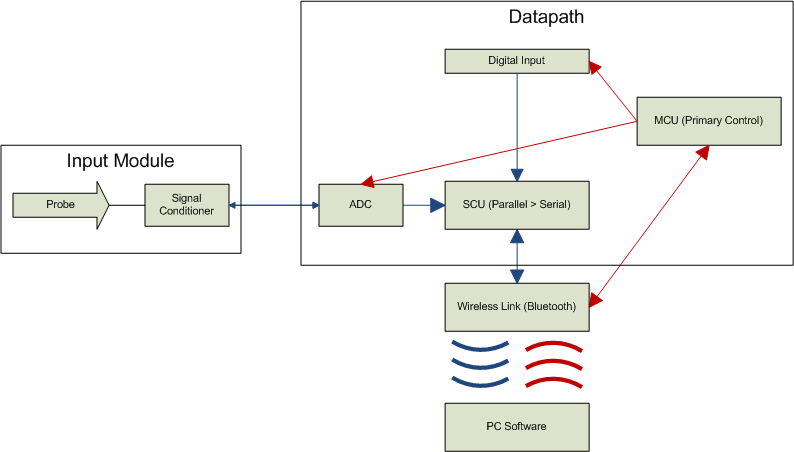
\includegraphics[width=4in]{../drawings/overview_block.png}
\label{fig:overall_block}
\end{figure} 

% Subsystem report for Power Supply system, typeset for the LaTeX processor.
\fancyfoot[R]{MM}
\section [Cost]{Cost Estimate}

\begin{table}[htb!]
\addtolength{\tabcolsep}{-4pt}
\caption{Capital Cost Estimate}
\small
\begin{center}
% Table generated by Excel2LaTeX from sheet 'Sheet1'
\begin{tabular}{p{1.5cm}|p{2cm}cccc|p{1cm}p{1cm}p{1cm}}

 Suppliers & Description &   Quantity & Supplier 1 & Supplier 2 & Supplier 3 &    Total 1 &    Total 2 &    Total 3 \\
\hline
\cite{web:jameco-price, web:digikey-price, web:newark-price} &  Resistors &         12 &     \$0.10 &     \$0.08 &     \$0.10 &     \$1.20 &     \$0.96 &     \$1.20 \\

\cite{web:jameco-price, web:digikey-price, web:newark-price} & Multiplexer &          1 &     \$1.09 &     \$1.58 &     \$1.58 &     \$1.09 &     \$1.58 &     \$1.58 \\

\cite{web:jameco-price, web:wflorida-price, web:newark-price} &     OpAmps &          4 &     \$0.25 &     \$0.20 &     \$0.29 &     \$1.00 &     \$0.80 &     \$1.16 \\

\cite{web:mouser-price, web:newark-price, web:futurelec-price} &        DAC &          1 &     \$3.49 &     \$3.44 &     \$3.50 &     \$3.49 &     \$3.44 &     \$3.50 \\

\cite{web:digikey-price, web:newark-price, web:futurelec-price} &     Diodes &          2 &     \$0.30 &     \$0.33 &     \$0.30 &     \$0.60 &     \$0.66 &     \$0.60 \\
\hline
\cite{web:caddell-burns-price, web:gowanda-price} & 68uH Inductor &          2 &     \$5.40 &          * &          * &    \$10.80 &    \$10.80 &    \$10.80 \\

\cite{web:wt32-price} & Bluegiga WT-32 &          1 &    \$89.95 &          * &          * &    \$89.95 &    \$89.95 &    \$89.95 \\

\cite{web:newark-price, web:mouser-price} & 1N5818 Schottky Diode &          2 &     \$0.14 &     \$0.09 &          * &     \$0.28 &     \$0.18 &     \$0.23 \\

\cite{web:lintech-price} & LT1073CN8-12 &          1 &     \$3.15 &          * &          * &     \$3.15 &     \$3.15 &     \$3.15 \\

\cite{web:lintech-price} & LT1073CN8-5 &          1 &     \$3.15 &          * &          * &     \$3.15 &     \$3.15 &     \$3.15 \\

\cite{web:mouser-price, web:resistor-price, web:digikey-price} &        LED &          1 &     \$0.90 &     \$1.49 &     \$0.78 &     \$0.90 &     \$1.49 &     \$0.78 \\

\cite{web:batt-price, web:batt-price2} & 3.7V Li-Ion Battery &          1 &     \$9.95 &    \$12.95 &          * &     \$9.95 &    \$12.95 &    \$11.45 \\

\cite{web:jameco-price, web:digikey-price, web:newark-price} &  Resistors &          3 &     \$0.10 &     \$0.08 &     \$0.10 &     \$0.30 &     \$0.24 &     \$0.30 \\
\hline
\cite{web:batchpcb} & Printed circuit board &          1 &    \$50.00 &          * &          * &    \$50.00 &    \$50.00 &    \$50.00 \\

\cite{web:jameco_atmel} & ATMega8515(L) &          2 &     \$4.58 &          * &          * &     \$9.16 &     \$9.16 &     \$9.16 \\

\cite{web:jameco_inv} &     74AC04 &          1 &     \$0.06 &          * &          * &     \$0.06 &     \$0.06 &     \$0.06 \\

\cite{web:jameco_inv} &    74AC245 &         10 &     \$0.09 &          * &          * &     \$0.89 &     \$0.89 &     \$0.89 \\

\cite{web:sparkfun} &    Headers &          2 &     \$2.95 &          * &          * &     \$5.90 &     \$5.90 &     \$5.90 \\
\hline
Totals &            &            &            &            &            &   \$191.87 &   \$195.36 &   \$193.86 \\
\hline
  &   * = cost data averaged         &            &            &            &            &            &            &            \\

\end{tabular}  
\end{center}
\label{tab:cost_est}
\end{table}
\fancyfoot[R]{NH}
\section{Implementation Schedule}
The implementation schedule for the Modular Wireless Diagnostics Tool is shown
in Figure \ref{fig:implement sched}. The schedule begins on January 2, 2010 and 
is organized in weekly increments. Because the system requires further testing,
the schedule includes three weeks of prototype testing and further design refinement.
Following this period, a two-week lead-time allowed for order and shipment of parts, 
and one week alotted for part assembly and final system testing. The total estimated
implementation time is 6 weeks.


\begin{figure}[bhp]
\begin{center}
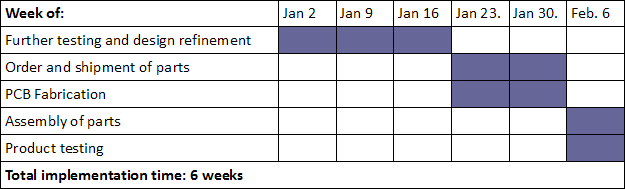
\includegraphics[scale=0.55]{../drawings/implement_sched.png}
\end{center}
\caption[Implementation Schedule]{Implementation schedule for the Modular Wireless
Diagnostics Tool.}
\label{fig:implement sched}
\end{figure}

\chapter{Subsystem Discussions}
%include subsystem reports here.
%like this: \include{report_name}
%report_name is the name of the .tex file, without the extension.
% Subsystem Report for the Analog Input Module system.
\fancyfoot[R]{WT}
\section[Analog Input]{Analog Input Module Subsystem}
\subsection{Description}
The purpose of the signal conditioning subsystem is to scale the analogue input
 to an appropriate level so that it can be read by the analogue to digital 
converter. The goal is to scale the output voltage to be between 0 and 5 volts 
and allow proper shifting and amplification via user interaction with the 
software. 

As per Figure \ref{fig:analog drawing}, this was implemented using 4 operational amplifiers, a digital to analogue converter, a multiplexer, resistors, and diodes. 741 operational amplifiers were chosen for this circuit because they are the most inexpensive op amps to purchase and their specs allow for them to be used in this circuit. A reference voltage of +/- 12 volts was used to supply these op amps, which allow for a maximum of +/- 22 volts\cite{ds:741 op amp}.

The input voltage is allowed to range from -12.7 volts to +12.7 volts. The 
diode and resistor configuration shown in drawing 201 assures the input voltage cannot vary outside of this range. These standard diodes and resistors were chosen because only basic diodes and resistors were needed and these components were very inexpensive. This input voltage is applied to the non-inverting input of an operational amplifier. The output of this op amp goes back to the inverting op amp, so it acts as a voltage follower\cite{bk:olia}.

Another voltage is produced from a digital to analogue converter. This voltage
 ranges from 0 to 5 volts. The purpose of the digital to analogue converter is
 to shift the signal up and down. The user controls this shift using the
 software on the computer. Because this requires communication with the micro
 controller, a digital to analogue converter was chosen with an 
I$^2$C interface. Consequently the PCF8591 was selected to 
produce a voltage ranging from 0 to 5 that goes into the non-inverting input 
of an op amp. This op amp also acts as a voltage follower.

These 2 voltages were each placed in series with a 10k resistor and both 
connected to the inverting input of another op amp. This op amp serves to 
amplify the voltage signal. Essentially the output from this op amp is the sum
 of the input and DAC voltages multiplied by the amplification[5]. The 4067
 analogue multiplexer is used to select the appropriate resistance. Like the 
digital to analogue converter, the multiplexer gets information from the micro
 controller and activates the desired output to use a resistor. These
 resistors vary from 10k ohms to 1M ohms to allow for different levels of 
amplifications. For example, for 2x amplification, the 20k resistor is used 
($20k/10k = 2x$ amplification) and this is multiplied by the sum of the 
earlier voltages\cite{bk:olia}.

The final op amp is used to scale the signal down to between 0 and 5 volts for 
the analogue to digital controller to read. An inverting op amp configuration 
is used with 3 volts going into the non-inverting input.
The output of this op amp is then sent to the analogue to digital converter.
Figure 201 and table 201 summarize the different parts of the circuit.

\subsection{Implementation}
Constructing the circuit is straight-forward and the connections can be seen 
from Figure \ref{sch:signal amp}. Setting up the circuit to be tested requires 
multiple voltage sources. Setting up the source voltages can be a little tricky.
Since the 741 op amps are not rail to rail, the +12 and -12 reference voltages 
must be supplied using 2 different voltage sources[1]. 

If the circuit is going to be implemented separately from the micro controller, another voltage source should be used as the voltage to the op amp by circle 
2 in figure 201. Another voltage source of 3 volts should be applied to the 
non-inverting input of the op amp by circle 6 in figure 201. Finally the input 
voltage should be applied to circle 1 in figure 201. Finding multiple power 
supplies is necessary before testing the unit as a whole. 
The feedback resistor of the op amp by circle 5 in figure 201 can be manually 
placed there instead of through the multiplexer if being tested without the 
micro controller. 

To start off, the voltage clamp of the diodes and resistors by circle 1 in 
figure 201 is tested. Use a multimeter to test the voltage before it reaches 
the first op amp. Adjust the input to points outside the + and -12.7 volts. 
The output should not be bellow -12.7 nor above +12.7 volts[1]. 
	Next, test the op amps by circles 2 and 3 in figure 201 and make sure the 
output voltage is equal to the input. Then record the voltage coming out of the
 op amp by circle 5 in figure 201 with 10k feedback. This should be 
approximately equal to the inversion of the sum of the input and digital to 
analogue voltages\cite{bk:olia}.
The feedback resistor of the op amp by (5) in Figure figure 201 can be manually
 placed there instead of through the multiplexer if being tested without the 
micro controller. 

The voltage clamp of the diodes and resistors by (1) in
 Figure\ref{sch:signal amp} should be tested first. Use a multimeter to test
 the voltage before it reaches the first op amp. Adjust the input to points 
outside the + and -12.7 volts. The output should not be below -12.7, nor 
should it be above +12.7 volts.

Next, test the op amps by circles 2 and 3 in figure 201 and make sure the 
output voltage is equal to the input. Then record the voltage coming out of 
the op amp by circle 5 in figure 201 with 10k feedback. This should be 
approximately equal to the inversion of the sum of the input and digital to 
analogue voltages\cite{bk:olia}. \begin{equation} V = -[V_{DAC} + V_{IN}]\end{equation}

If this is correct, finally test the output voltage coming out of the op amp by
 circle 6 in . Put the input voltage to the max of 12.7 and the DAC 
voltage to its max of 5. This should yield an output of 0. Then set the input 
voltage to -12.7 and the DAC voltage to 0. The output voltage should be around 
5 volts. Any other input voltage levels should show an output voltage between 0 and 5 and be approximately:

\begin{equation}\label{vout}V_{OUT} = 3 - .16447[V_{DAC} + V_{IN}]\end{equation}

When testing the circuit, the actual output voltage did not match up with the 
theoretical output described by \eqref{vout}. Table \ref{tbl:analog input data}
 shows the different input voltages and the resulting outputs of the
 theoretical and actual voltages.

Although these results did not match up precisely with what was expected, they 
are still within the range of the analogue to digital converter to read. They 
were just scaled to different values.

\subsection{Fault Analysis}
There are several obvious but overlooked reasons as to why this circuit 
would not operate properly. Understanding the op amp is key to knowing what is
 wrong. During preliminary testing, the op amp was not showing any output
 voltage when constructed as a voltage follower. After many attempts, no output
 voltage could be obtained. Finally the op amp was moved to another part of
 the breadboard and it operated correctly right away. A part of the breadboard
 used was not operating correctly. A faulty breadboard can be tested with a 
multimeter to make sure the connections are properly working.

It is possible to ruin the diodes or op amps if excess voltage is give to
 them. If the diodes are facing the wrong direction they will also not operate
 properly. If there as any doubt of the components not working correctly, get
 new parts to replace them. The diodes and op amps are cheap so it would not 
cost very much to use another one.

If the actual voltages and theoretical voltages are varying, it could be 
because of variances in each device. Make sure to use resistors with gold (5\%)
 tolerances. Also, the exact measurements should be obtained before plugging
 them into the equations used, not the theoretical values.
	It is recommended to change the parameters surrounding the final op amp to 
alter the output. Changing the resistances of the negative feedback and the
 voltage level of the non-inverting output should be done to alter the output.

\subsection{Cost}
20 components must be obtained to build this circuit. Each part is shown in 
drawing 201 and table 203. 12 resistors are used. 3 1k resistors are used,
 with 2 for the voltage clamp and 1 for the final op amp. 1 6.2k resistor is
 used for the final op amp. 3 10k resistors are used with 2 being placed after
 each voltage follower and the other in the variable resistance feedback. The 
remaining 5 are used in the variable resistance feedback with values of 20k,
 50k, 100k, 500k, and 1M ohms.
	2 1N4001 diodes, 4 741 op amps, 1 4067 multiplexer, and 1 digital to
 analogue converter are also used.

\begin{figure}[hbp]
\caption{Photograph of implemented signal conditioner on breadboard}
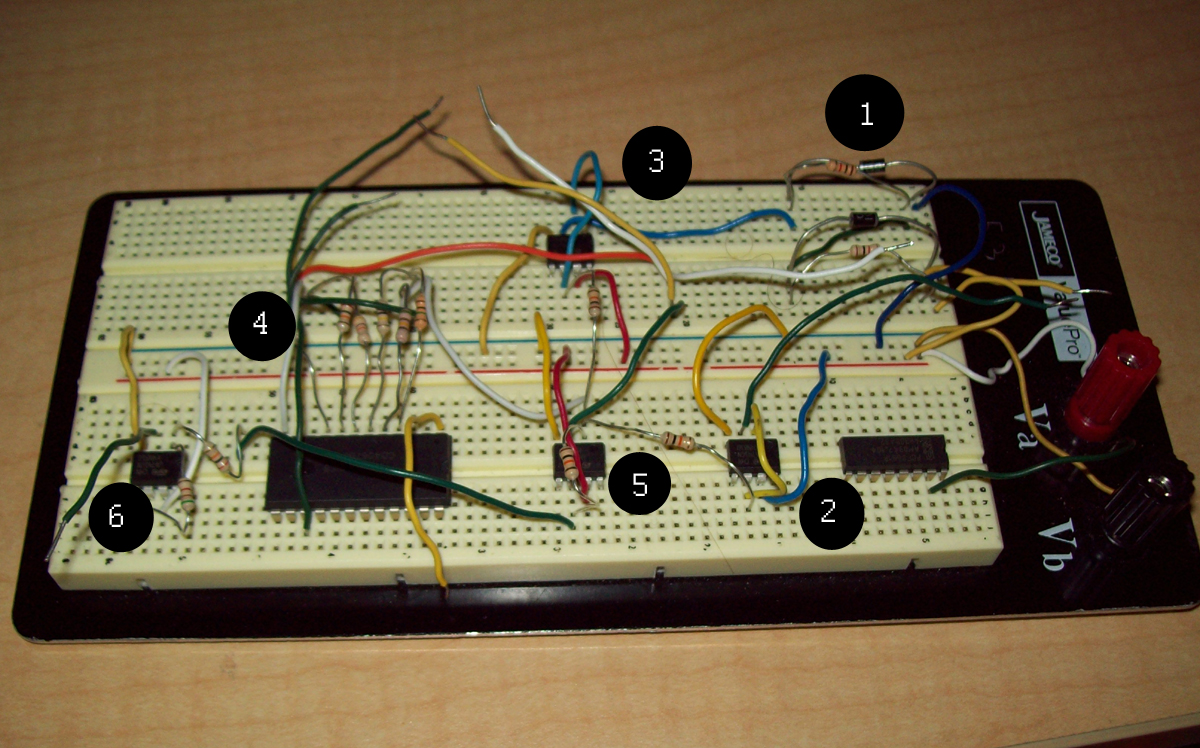
\includegraphics[width=5in]{sub_analog_hw.jpg}
\label{fig:analog breadboard}
\end{figure}

\subsection{Performance Data}
\begin{table}[hbp]
\caption[Test Results]{Expected and Actual Results (With 1x amplification)}
\begin{center}
\begin{tabular}{c| r @{.} l r @{.} l r @{.} l}  
	Input Voltage & \multicolumn{2}{r}{DAC Voltage} &
	\multicolumn{2}{r}{Theoretical Voltage} &
	\multicolumn{2}{r}{Actual Voltage} \\ \hline
	12 & 7 & 5 & 0 & 09 & 1 & 4 \\ \hline
	10 & 0 & 3 & 0 & 86 & 1 & 9 \\ \hline
	2  & 0 & 4 & 2 & 01 & 3 & 2 \\ \hline
	-12 & 7 & 0 & 5 & 08 &5 & 1 \\
\end{tabular}
\end{center}
\label{tab:analog input data}
\end{table}



% Subsystem report for Power Supply system, typeset for the LaTeX processor.
\fancyfoot[R]{MM}
\section [Power]{Power Subsystem}
\subsection{Description}

The power system \index{power} provides reliable, standalone power to all other hardware subsystems. The design supports three different voltage levels as the ATMEGA8518 MCU, analog signal conditioner, and WT32 bluetooth module all require different reference voltages. The source has the flexibility to operate from battery or, when interfaced with a standard USB port, charge the in-system battery and provide uninterrupted power when switching between the two.  

\subsection{System Power Requirements}

Each subsystem requires a different supply voltage as shown in Table \ref{tab:power requirements}. 
\begin{table}[bhp]
\caption[Power Requirements]{Recommended DC operating voltages for ATMEGA8515\cite{ds:ATMEGA8515} and WT32\cite{ds:WT32}}
\small
\begin{center}
\begin{tabular}{l| c c}
\setlength{\tabcolsep}{1pt}
	Device     & Minimum   & Maximum \\\hline
	ATMEGA8515 & 2.7 V     & 5.5 V   \\             
	Analog Signal 
	Conditioner& -12 V     & +12 V\\            
  \small{ADC}& N/A		   & Quiet 3 V\\
	WT-32      & 2.5 V     & 4.4 V            
\end{tabular}
\end{center}
\label{tab:power requirements}
\end{table}

\subsection{Battery}

Taken into consideration are three potential in-system, rechargeable battery\index{battery} supply options: Alkaline, NiMH, or Li-Poly. For some of the basic metrics taken into consideration see table \ref{tab:battery comparison}. Alkaline batteries in series are not a bad option as it would provide the 3V DC source necessary for the MCU and a similar arrangement could provide power for the other sub-systems as well. The issue with this approach is efficient in-system charging. As with all of the rechargeable batteries considered, use of multiple-cells in a charging system require some intelligent monitoring of each cell to assure that no cell is too far out of sink which can result in overcharging or reverse-charging as a charged cells will rapidly discharge into the uncharged cell. Overcharging can, at the least, damage the battery if not resulting in a dangerous explosion due to an un-containable build up of gaseous bi-products. Another drawback to Alkaline is that voltage output degrades linearly over time which is unfavorable for high-drain electronics. 

NiMH batteries maintain a more consistent voltage over time but have a relatively low efficiency. The best battery solution for this design is the Li-Poly as it not only has a superior efficiency, a single cell outputs a nominal voltage of 3.7 V DC which is acceptable for directly powering the WT-32 bluetooth module. As an added bonus, the WT-32 has a built-in battery charging application as it is often utilized with integrated single cell Li-Poly batteries (i.e. - bluetooth headsets, cell phones). 
  
\begin{table}[bhp]
\caption[Common Battery Types]{Comparison of Common Battery Types\cite{web:bat-tech}}
\small
\begin{center}
\begin{tabular}{l| c c c}
\setlength{\tabcolsep}{1pt}
	Battery     & Single Cell Voltage   & Efficiency & No. of Cycles\\\hline
	Alkaline & 1.5 V                    & 99.9\%        & 100 - 1000\\             
	NiMH     & 1.2 V                    & 66.0\%        & 1000      \\            
  Li-Poly  & 3.7 V		                & 99.8\%        & 500 - 1000 
\end{tabular}
\end{center}
\label{tab:battery comparison}
\end{table}

\subsection{DC/DC Converter}

The Li-Poly battery integrated with the WT32 bluetooth module provides a level 3.7 V DC source which must be re-leveled and distributed to the other sub-systems with as little ripple as possible. Component selection for this application takes into consideration the need for high efficiency. DC-DC converter packages are cheap and readily available so the alternative of building a custom supply is unnecessary. Low-power DC DC converters come in two basic varieties: fixed and adjustable. The adjustable converters feature a built-in gain setting resistor for the internal op-amp and in the case of the LT1073, only three passives are required to configure the device. Refer to figure \ref{fig:general step-up} for an example of the the fixed output implementation.

\begin{figure}[hbp]
\centering
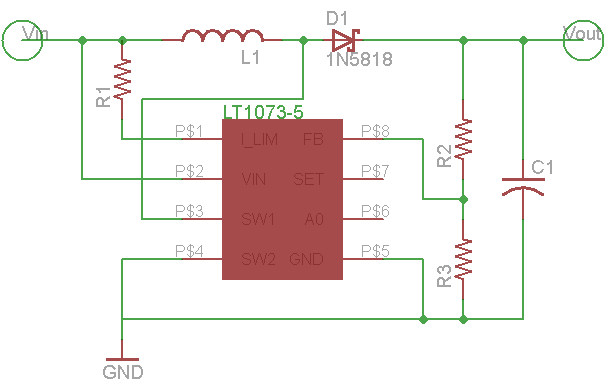
\includegraphics[scale=0.95]{../drawings/power_gen_fixed.png}
\caption[LT1073 Fixed Output Configuration]{LT1073 general fixed output configuration\cite{ds:lt1073}}
\label{fig:general step-up}
\end{figure}

The datasheet for the LT1073 includes straightforward equations for deciding what values are necessary for the passive components depending on the desired output voltage and current. The standard configurations for the fixed voltage step-up converters from 3V to 5V and 12V are sufficient if the components are up to specification. Namely, the inductor must be able to buffer the input voltage when switching on or off. The inductor must have a low resistance to avoid wasting energy and must not saturate. 

\subsection{Prototyping}

Prototyping the power subsystem is most effectively accomplished using protoboard and a wire wrapping tool. Using DIP wire wrap sockets for the passives required for the LT1073 DC-DC converter allows for fast teaking if output voltages are not within expected tolerances. The working prototype currently supports the WT32 and ATMEGA8518 power requirements. This prototype may also be powered either via the integrated Li-Poly battery cell or standard USB connection. The Li-Poly battery leverages the WT32 built-in charging system. Future expansions will include the +/- 12V DC power support for the Analog Input Module as shown in Figure \ref{fig:final_power_schematic} .

\begin{figure}[hbp]
\centering
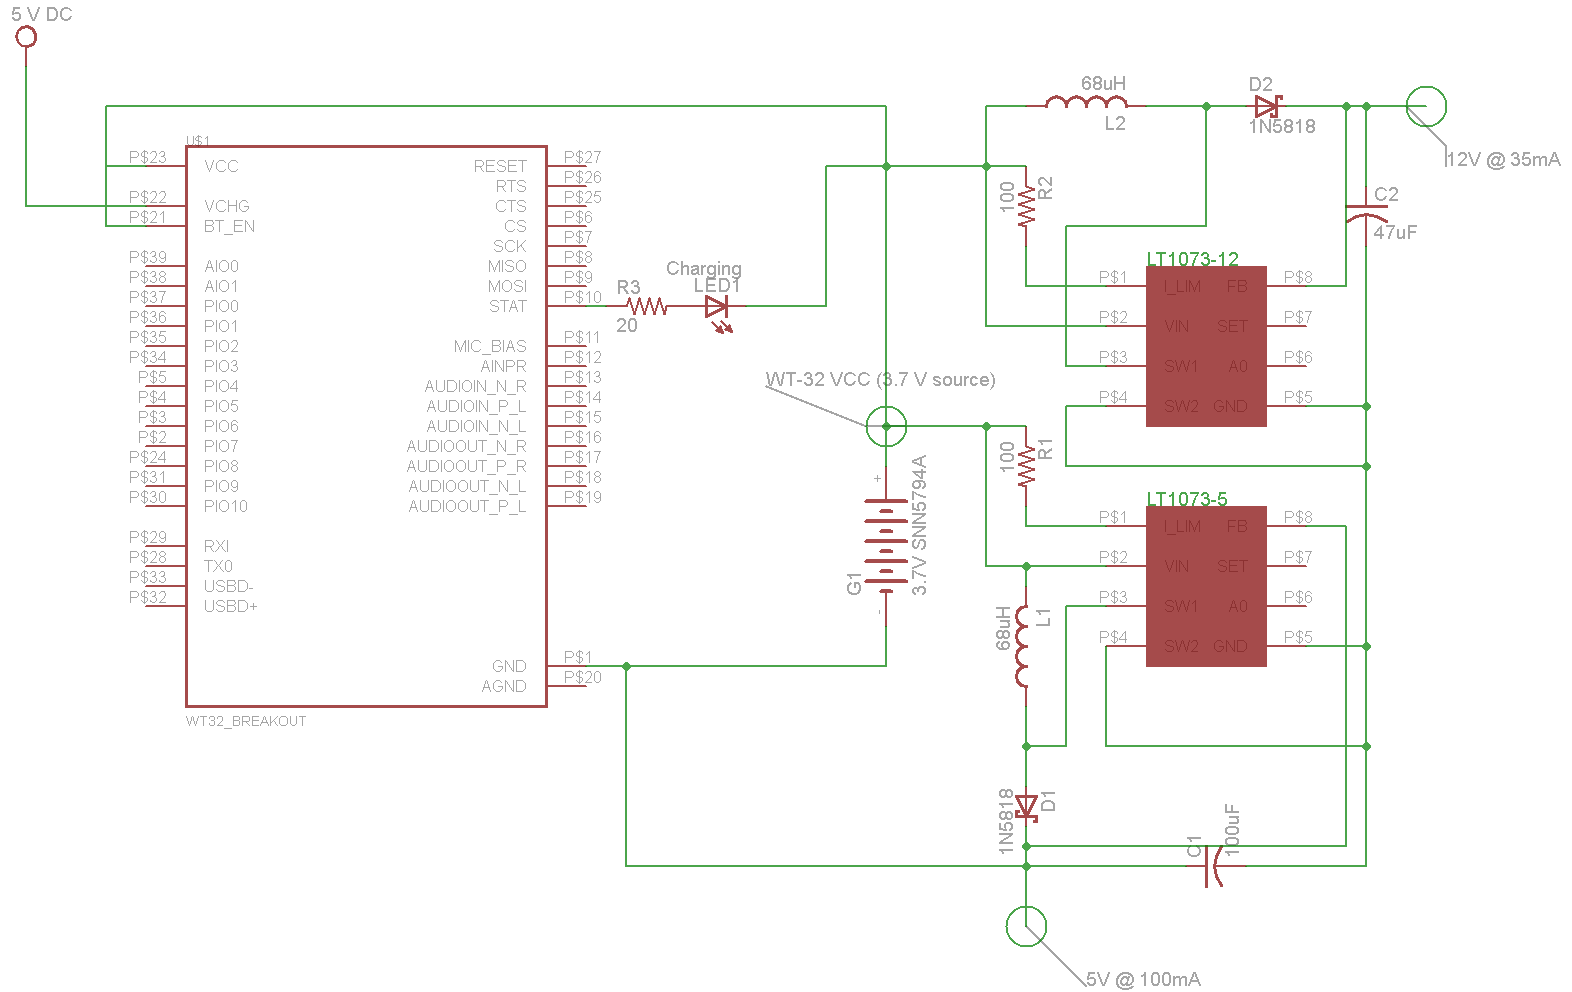
\includegraphics[scale=0.75]{../drawings/power_final_sch.png}
\caption[Power Supply]{Power supply prototype schematic}
\label{fig:final_power_schematic}
\end{figure}   

It is important to note that while prototyping does not require close quarters for the necessary components, a production model may require a toroidal instead of rod-type inductor in order to reduce the effects of EMI on the analog circuitry. Also, in the interest of cost, simple electrolytic capacitors are used instead of high end Tantalum capacitors. 1N5818 Schottky diodes are suggested for the LT1073 as they have a low forward voltage drop and switch quickly. Extensive trials are still required for this prototype inorder to establish actual operating battery life, overall battery life, and possible variation due to noise. The critical power drawing component is the Acquisition Unit which may be characterized by the ATMEGA8515. Refer to Table \ref{tab:battery comparison} to view a best/worst case estimates considering only the two MCU in use. It is notable that it would be very unlikely for both MCUs to be operating constantly. 

\begin{table}[bhp]
\caption[Estimated Operating Time]{Power consumption estimate -  assuming 30\% idle time\cite{ds:ATMEGA8515}}
\small
\begin{center}
\begin{tabular}{l|llll}
\setlength{\tabcolsep}{1pt}
	Device Operation & Supply (Ib) & Active Current(Id) & Idle Current(Id) & Estimated battery\\ 										&				 &													& &life = (Ib / Id) x 0.7\\\hline
	Li-Poly          & 780mAh &													 & &											\\
	One MCU          &        & 12 mA                    & 5.5 mA      & 54.33 hr \\
	Both MCUs        &        & 24 mA                    & 11.0 mA     & 38.01 hr \\    
  Average          &        & 18 mA		                 & 16.5 mA     & 31.11 hr 
\end{tabular}
\end{center}
\label{tab:battery comparison}
\end{table}

\subsection{RoHS Compliance}

Not all components in the power supply prototype are RoHS (Restriction of Hazardous Substances) compliant as many rod-type passives may contain lead. RoHS restricts the use of lead, mercury, cadmium, hexavalent chromium,and polybrominated diphenylether in electronics. Although this standard is not yet enforced in the United States, it may be soon. It is recommended that any production model only use RoHS compliant materials in the interest of a globally accepted product.

\subsection{Power Supply Cost}

The implementation of the power supply requires the purchase of several ultimately uncessary components for the purposes of testing and to avoid prototyping delays in the event that a component is faulty or damaged. See Table \ref{tab:power_imp_cost_est} for cost estimates to implement the design.

\begin{table}[bhp]
\caption[Implementation Cost]{Power System Implementation%
Cost\cite{web:caddell-burns-price} \cite{web:wt32-price} \cite{web:resistor-price} \cite{web:cap-price}}
\small
\centering
% Table generated by Excel2LaTeX from sheet 'Sheet1'
\begin{tabular}{l|l|l|l|l}
\setlength{\tabcolsep}{1pt}
Product \# & Description & Quantity & Price/Unit & Total \\\hline
WRL-08952  & Bluetooth� Breakout - Bluegiga WT-32  &          1 &    \$89.95 &    \$89.95 \\

    1N5818 & Schottky Diode &         20 &     \$0.14 &     \$2.84 \\

    1N4933 & Fast Recovery Power Rectifier &         10 &     \$0.05 &     \$0.53 \\

106CKR050M & Electrolytic Capacitor &         10 &     \$0.05 &     \$0.45 \\

COM-00526  & Voltage Regulator - 3.3V  &          1 &     \$1.95 &     \$1.95 \\

COM-00527  & Voltage Regulator adjustable &          1 &     \$1.95 &     \$1.95 \\

 LT1073CN8  & MicroPower DC-DC Converter &          2 &     \$3.15 &     \$6.30 \\

LT1073CN8-12  & MicroPower DC-DC Converter (12 VDC FIXED) &          2 &     \$3.15 &     \$6.30 \\

LT1073CN8-5  & MicroPower DC-DC Converter (lead free) &          2 &     \$3.15 &     \$6.30 \\

   7300-11 & Caddell-Burns 68uH inductor &          2 &     \$5.40 &    \$10.80 \\
   271-308  & 100 pc resistor assortment & 					1 &			\$6.49 &    \$6.49 \\
   276-309  & 5mm red LED								 &					1 &			\$1.49 &    \$1.49 \\
   SNN5794A & Motorola battery pack			 &					1	&			on hand&    onhand \\
Grand Total & & & & \$133.40\\
\end{tabular}   
\label{tab:power_imp_cost_est}
\end{table}

The actual cost for production is much less than prototype implementation as optimal components have been chosen. This cost is further lessened due to the likelihood that large quantities will be ordered, however, the proto-type cost estimate shown in Table \ref{tab:power_prod_cost_est} only assumes a minimum number of components required for a single build.

\begin{table}[bhp]
\caption[Production Cost]{Power System Production Cost \cite{web:caddell-burns-price} \cite{web:cap-price} \cite{web:batt-price}}
\small
\centering
% Table generated by Excel2LaTeX from sheet 'Sheet1'
\begin{tabular}{l|l|l|l|l}
\setlength{\tabcolsep}{1pt}
    Part \# & Description &   Quantity &   Per/Unit & Total Cost \\\hline

WRL-08952  & Bluetooth� Breakout - Bluegiga WT-32  &          1 &    \$89.95 &    \$89.95 \\

    1N5818 & Schottky Diode &          2 &     \$0.14 &     \$0.28 \\

    G13440 & 100uF dipped Tantalum Capacitor &          1 &     \$1.00 &     \$1.00 \\

     G7102 & 47uF dipped Tantalum Capacitor &          1 &     \$1.00 &     \$1.00 \\

LT1073CN8-12  & MicroPower DC-DC Converter (12 VDC FIXED) &          1 &     \$3.15 &     \$3.15 \\

LT1073CN8-5  & MicroPower DC-DC Converter (lead free) &          1 &     \$3.15 &     \$3.15 \\

   7300-11 & Caddell-Burns 68uH inductor &          2 &     \$5.40 &    \$10.80 \\

   276-309 & 5mm red LED &          1 &     \$1.49 &     \$1.49 \\

   271-308 & 100 pc resistor assortment &          1 &     \$6.49 &     \$6.49 \\

  SNN5794A & 3.7 V Lithium Ion Rechargeable Battery &          1 &     \$9.95 &     \$9.95 \\
  Grand Total & & & & \$127.26\\

\end{tabular}  
\label{tab:power_prod_cost_est}
\end{table}

% Subsystem report for Datapath control system, typeset for the LaTeX processor.
% Copy the next line and put your initials instead of JL.
\fancyfoot[R]{JL}
\section[Datapath Control]{Acquisition Unit Datapath Control}
% Description of function or purpose
\subsection{Description}
For the data acquisition hardware, a flexible base was needed to manage the 
flow of data from the analog or digital input modules to the host PC. It was 
also desired to allow the host PC to manage the configuration of the input 
modules themselves. The datapath control subsystem regulates the flow of data 
from the input modules\index{input modules} and serializes it for output to 
the host PC software. It provides a multiplexed bus for analog and/or 
digital interface modules and also provides a control interface for those 
modules. The bus width was set at 10 bits, which was the minimum size for
 accepting output from the analog input module designed for use with this 
datapath.
\subsection[Tradeoffs]{Design Decisions and Tradeoffs} 
Table \ref{tab:control comparison} lists an overview of the options considered
 for the datapath control subsystem. Cost refers to the per-unit cost of a 
given solution, Complexity is the amount of up-front design work that would
 need to be done to achieve basic functionality. TTL Logic and FPGAs are, for
 these considerations, similar. Both require much work to achieve some basic
 functionality but had very few limits in the the types of solutions that
 could be realized. FPGAs have an additional advantage over basic logic gates
 in that they are able to be relatively easily reconfigured or updating, which
 would make prottotyping simpler. However, both solutions low-level
 implementations were considered to be too time-inefficient for this design.
 A general purpose "bare" microprocessor was also considered, but was quickly
 dismissed for similar reasons as FPGAs - the infrastructure required to get
 a general microprocessor functioning was also considered time-inefficient.

\begin{table}[bp]
\caption[Controllers]{Comparison of different control methods}
\begin{tabular}{l| c c c c c c}
		\multirow{2}{*}{\small{Control Type}} & \multirow{2}{*}{\small{Cost}} 
		& \multirow{2}{*}{\small{Complexity}} & \multirow{2}{*}{\small{Flexibility}} 
		& \multirow{2}{*}{\small{Speed}} 
		& \small{Time}\\
		&&&&&\small{Required}\\ \hline
		\small{Basic logic}  &     &      &      &     & \\
		  \small{gate chips} & \small{Low} & \small{High} & \small{High} & \small{Low} & \small{V. High} \\ 
		\small{FPGA} & \small{Average} & \small{High} & \small{High} & \small{Average} & \small{High}  \\
		\small{Microprocessor} &\small{ Average} & \small{High} & \small{Average} & \small{Average}
		 & \small{Average} \\
		\small{Microcontroller} & \small{Low} & \small{Low} & \small{Average} & \small{Average} & \small{Low} \\
\end{tabular}
\label{tab:control comparison}
\end{table}

Microcontrollers, however, are ideal for this type of application: they provide
 a flexible base and generally come packaged with different interfacing 
subsystems of their own for a low cost. In addition, many microcontrollers 
have a C compiler ported for their architecture, as well as the ability to
 reprogram them in-system. Table \ref{tab:MCU capabilities} outlines some of
 the capabilties of two microcontrollers that had been under consideration.
 While the the two devices are very similar, the Atmel MCU was chosen for its
 more flexible layout, multiple integrated interfaces, and the availability
 of a mature port of the GNU C Compiler for the device (and its family). The 
PIC required the use of the vendor-supplied compiler and IDE.
\begin{table}[bhp]
\caption[Atmel and PIC MCUs]{Comparison of Atmel ATMega8515 and PIC18F1220}
\begin{tabular}{l| c c c c c c}
\setlength{\tabcolsep}{1pt}
	       &      & \small{Pin}  & \small{Maximum} & \small{Ease}   &            &         \\
	\small{Device} & \small{Cost} & \small{Count} & \small{Speed}  & \small{of Use} 
	& \small{Interfaces} & \small{Features}\\\hline
	\multirow{3}{*}{\small{ATMega8515}} & \multirow{3}{*}{\small{Low}} & \multirow{3}{*}{\small{40}}
	& \multirow{3}{*}{\small{20Mhz}} & \small{High} 
	& \small{SPI,} & \small{Timers}\\
	           &     &    &       &      &\small{USART} & \small{External}\\
	& & & & & &\small{Memory}\\\hline
	\small{PIC18F1220} & \small{Low} & \small{18} & \small{40Mhz} & \small{Average} & 
	\small{USART} & \small{Timers} \\
	           &     &    &       &      &  & \small{10-bit ADC}\\
\end{tabular}
\label{tab:MCU capabilities}
\end{table}

The bus interface features two input ports and one output port. To effectively
 switch between the two inputs, those connections must be tri-stated. Three 
74-series tri-state buffers were considered: the 74*244, the 74*245, and the 
74*621. Table \ref{tab:buffer comparison} outlines the key differences with 
the components considered. Ultimately, a 74*245 chip was selected for its 
flexibility and that there was a supply already on-site. 74*621s were found 
to be difficult to source in low quantites for a prototype. 74*244s could be 
used as well with some minor changes in glue logic, as well as 74*621s.

\begin{table}[bhp]
\caption[Buffer Comparison]{Comparison of different tri-state buffers}
\small
\begin{center}
\begin{tabular}{l| c c c c}
\setlength{\tabcolsep}{1pt}
	Device & Width & Bi-Directional & Cost & Availability \\\hline
	74*244 & 8     & No             & Low  & High\\
	74*245 & 8     & Yes            & Low  & High\\
	74*621 & 8     & Yes            & Low  & Low
\end{tabular}
\end{center}
\label{tab:buffer comparison}
\end{table}

\cite{ds:ATMEGA8515}

\fancyfoot[R]{DP}
\section[Wireless Communication]
\subsection{Overview}
For communications between the device and the users computer it was decided 
that a wireless connection would be used.  This is because it would be more 
convenient for the user to be able to connect to the device wireless instead of
 being tied down by the physical connection.  There were three choices for use:
 the WT 32 Bluegiga made by Bluegiga Technologies, the BG203 made by SparkFun, 
and the Roving Networks Bluetooth made by Roving Networks.  The first thing 
that is to be taken into consideration is the cost of each chip. Look at 
Table\ref{tab:bt_prices} to see the difference in price.

\begin{table}[hbp]
\caption{Comparison between different communications modules \cite{web:wt32-price}\cite{web:bg203-price}\cite{web:roving-price}}
\begin{tabular}{l | c c } 
	System Name & Packaging & Price \\\hline
	WT32 Bluegiga Breakout & Dual-Inline & \$89.95/unit \\
	BG203 & & \$54.95 \\
	Roving Networks & & \$59.95
\end{tabular}
\label{tab:bt_prices}
\end{table}

If the decision was to be made based purely on the price of the chip then the 
BG 203 would have been chosen but it was not.  This is because out of all three
 of these chips the BG203 was not a breakout chip.  A breakout chip is a chip 
that will allow the user to program the chip further to better suit the users 
needs.  Without this feature the BG203 would have had limited use.

The choice of the WT32 Bluegiga over the Roving Networks Bluetooth comes from 
the features of the chip.  Now, there are many common features of the two chips
 like how they are both qualified bluetooth modules and both work on 3.3 volts.
  But what made the WT32 more preferable was the fact that ``A host processor 
can control the functionality with ASCII commands via UART or USB 
interface'' meaning that a program can be made to give the chip commands 
instead of having to do it manually\cite{web:wt32-price}.  This is why that 
even though the WT32 Bluegiga is the most expensive out of all the chips it is 
the chip that is best for this type of project.

The program that was written for this works by sending the command over the USART.  This is done simply by having a set of commands that were taken from the 
IWRAP user's guide.  All the user needs to make sure of is that the WT32 is in data mode and then all the user has to do is type in the command they want to use and then the program will send it to the chip and then it is done.

%Subsystem report for the PC Software subsystem
\fancyfoot[R]{NH}
\section[PC Software]{PC Software Subsystem}
\subsection{Description}
	The PC Software subsystem is responsible for performing two major tasks of 
the PC Diagnostics Tool. The first task is the acquisition of data from the 
Acquisition Unit / Datapath Control subsystem and subsequent storage of data on 
the end-user's PC. The second task is the provision of a display/control 
interface for an end-user operating device. A user must be able to send the 
necessary signals to the PC Diagnostics Tool hardware to control the output of 
the tool, and he or she must have a method of organizing and displaying 
acquired data.

A block diagram of the subsystem is shown in Figure \ref{fig:pcsoft sub diagram}


\begin{figure}[bhp]
\begin{center}
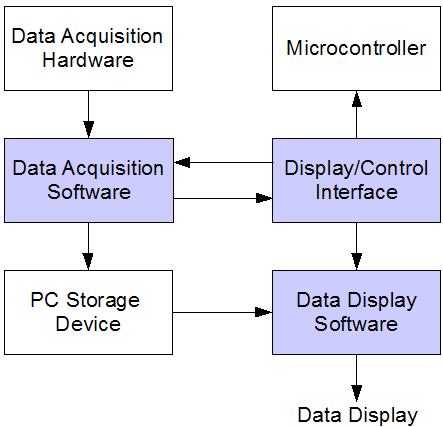
\includegraphics[scale=0.75]{../drawings/pcsoft_sub_diagram.png}
\end{center}
\caption[PC Software Block Diagram]{Block diagram of the PC Software Subsystem. White blocks
are not part of the subsystem.}
\label{fig:pcsoft sub diagram}
\end{figure}



\subsection[Design Decisions]{Design Decisions}
\subsubsection[Software Packages]{Software Packages}
There are two possible approaches to writing software that addresses both of 
these needs. The first is to utilize proprietary software development 
environments such as Matlab or Labview that bundle together data acquisition 
and Graphical User Interface (GUI) functionality in a relatively easy-to-use 
software package. The second is to manually build custom software to implement 
these functions.

The first approach considered was to use a proprietary signal processing 
environment. Perhaps the two most popular software packages in this area are 
Labview and Matlab. Labview is a development environment produced by National 
Instruments. Its base package offers user-friendly GUI development tools, ample 
drivers for data acquisition into the PC and even some signal processing 
functionality \cite{web:labviewbase}. Matlab is a widely-known computing 
environment for science and engineering applications with extensive signal 
processing functionality, GUI-development tools and a data acquisition toolbox 
for acquiring data into the PC \cite{web:matlab}. In other words, both packages 
offer exactly the needed functionality for this subsystem.

These features come at a price, however. The Labview base package costs 
\$1249 \cite{web:labviewbase}, while Matlab costs \$500 for a single-user license with an 
additional \$200 cost for the Data Acquisition Toolbox \cite{web:matlab}\cite{web:matlabdaq}. 
Furthermore, the nature of development environments like Labview and Matlab mean that 
developing a solution in either would result in a user interface that is only usable in 
Labview or Matlab. This means that end-users would be required to have working 
copies of whichever environment was used to develop the UI. Since hobbyists are 
the target market for othe PC Diagnostics Tool, it is not reasonable to expect 
that every user will possess a copy of Matlab or Labview, and it is even less 
reasonable to assume that every user would purchase a copy in order to use the 
GUI. Building standalone applications in either environment is possible, but it 
comes at further cost: the Labview Application Builder for Windows, at \$999 \cite{web:labviewbase} 
or the Matlab Compiler, at \$500 \cite{web:matlabcompiler}. 

With these cost considerations in mind, a proprietary solution was ruled out. 
The next options explored were programming languages and software packages that 
were inexpensive or free and could be used to implement the PC software. It was 
first necessary to break down the two tasks of the subsystem to understand what 
was required. A break-down of necessary functionality required to implement each
 task is shown in Table \ref{tab:required functionality}.


\begin{table}[bhp]
\begin{tabular}{l | p{7cm}}
	Task & Necessary functionality \\ \hline
	Data acquisition and storage & Serial port communications library, File I/O \\ \hline
	Display/control interface & Serial port communications library, GUI library, 
	Signal/waveform plotting
\end{tabular}
\caption[Software functionality]{PC Software tasks broken down by the necessary 
functionality to perform each.}
\label{tab:required functionality}
\end{table}


Of the required functionality, nearly every modern programming language has a 
capacity for serial port communications, file I/O and building GUIs, so the deciding 
factor would lie elsewhere. Some deciding factors were brainstormed, and languages were 
evaluated based on cost, ease of implementation and whether or not the resulting 
software would work on different operating systems (i.e. whether it was ``cross-platform'').  
Programming languages considered were C++, Java, and Python. 

The language comparison performed is shown in Table \ref{tab:languages features}. 
Due to non-availability of concrete data, performance of all three languages was 
considered to be ``good-enough'' for the software's purposes. All three languages here are 
widely-used, and considering again the target market of hobbyists, it can be expected 
that the languages are optimized enough for the performance needed. In considering the 
ease of implementation for each language, it was found that all the languages had online 
documentation available as well as a serial port library. The only criteria on which they
differed was the ``level'' of the language. Programming languages can be classified by what 
level the code required to perform a given task is abstracted away from the low-level 
hardware details of accomplishing the task, with high-level languages being farther 
abstracted from the details \cite{web:suranathesis}. Higher level languages are therefore 
easier to implement code with because the language compile or interpreter handle things 
like memory management and CPU operations.


\begin{table}[bhp]
\begin{tabular}{l | c | p{6cm} | c}
	Language & Cost & Ease of implementation & Cross-platform? \\ 
	\hline
	C++ & Free & Online documentation, serial port library, medium-level language \cite{web:cpptut}\cite{web:cppserial} & No \\ 
	\hline
	Java & Free & Online documentation, serial port library, medium-level language \cite{web:javaapi}\cite{web:javaserial} & Yes \\
	\hline
	Python & Free & Online documentation, serial port library, high-level language \cite{web:pydoc}\cite{web:pyserial} & Yes \\
\end{tabular}
\caption[Language features]{Comparison of programming language features.}
\label{tab:languages features}
\end{table}


After careful consideration of each language's features, it was decided to use Python as 
the programming language. Choosing C++ has no obvious benefits while having the exclusive 
drawback of not being cross-platform, and while Java has, for the purposes of this subsystem, 
essentially the same features as Python, a Python implementation should be easier because of 
its status as a high-level programming language.

For the signal/waveform plotting, it was decided from the beginning that, given the target 
market of hobbyists, real-time data display would not be necessary. Furthermore, many 
hobbyists using the PC Diagnostics Tool will have some technical background in engineering, 
and perhaps even some experience with computation software like Matlab. It seems reasonable, 
then, to perform the data plotting in a numerical computational environment in order to 
allow users to easily extend whatever functionality is provided by the default PC software. 
GNU Octave, a free, open source, Matlab-like numerical computing software package, provides 
such an environment \cite{web:octave}.

A list of software packages used for PC Software subsystem is shown in Table \ref{tab:software packages}. 
Python and GNU Octave have been previously discussed. PySerial is a cross-platform serial 
communications library for Python, and pywin32 is a Windows 32 API library for Python which is 
required for pySerial to work on Windows. All software packages are free and open source.


\begin{table}[bhp]
\begin{tabular}{l | p{8cm}}
	Software Package & Description \\ \hline
	Python & Programming language used to implement data acquisition and interface software. \\ 
	\hline
	pySerial & Serial port communications library for Python. \\
	\hline
	pywin32 & Windows 32 API library for Python, required for pySerial on Windows \\
	\hline
	\multicolumn{2}{l}{Total cost: \$0} \\
\end{tabular}
\caption[Software packages]{Software packages utilized by the PC Software subsytem, along with total cost.}
\label{tab:software packages}
\end{table}


\subsubsection[Software Implementation]{Software Implementation}
In order to facilitate the necessary software tasks outlined in Figure 
\ref{fig:pcsoft sub diagram}, some design options had to be sifted through. Specifically, 
how the data acquisition would be achieved. In order to prevent the act of data 
acquisition from tying up the resources of the user interface, it is necessary to launch 
the data acquisition software in a separate sub-process. This, however, introduces a 
problem of how the interface process and the data acquisition process will communicate with 
each other. There exist, however, several techniques that enable communication between 
processes, which are aptly called inter-process communication (IPC) techniques. Pipes are 
perhaps the simplest method among these, but it turns out that a necessary operating system 
call named \textit{fork()} does not work on Windows \cite{web:windowsfork}. Furthermore, 
after much testing, the Python workaround for this inconsistency was found to be non-functional. 
Sockets are the next-best choice because, while they are not the simplest method, sockets can
 communicate over a network. This opens up the possibility of the data acquisition software 
running on a separate machine from the interface, which could be useful for a few different 
applications.

There is another problem that the PC Software must solve: when using a Python application to 
implement the user interface and GNU Octave to perform data plotting, it becomes impossible to 
utilize IPC to enable communication between the two. Being that GNU Octave is open source, one 
solution is to use Octave's C++ headers and a software package called Simplified Wrapper and Interface
 Generator (SWIG) to directly call  GNU Octave's plot functions from the interface itself \cite{web:swig}. 
This turned out to not be feasible due to copyright issues: GNU Octave is distributed under the GNU 
GPL, a copyright license that requires any code that links to GPL'd code to itself be released under 
the GNU GPL \cite{web:gnugpl}. In the interests of potential future commercialization, it was desired 
that the code to the PC Software not become open source. A simple, effective solution to this is to 
use Python's \textit{subprocess} module to launch an instance of Octave that executes a data display 
script. Before the launch, data is written to a control file that the Octave script later reads 
to find out which data should be displayed. This enables on-demand data plotting without resorting 
to using GNU Octave headers.

\subsection[Software Design]{Software Design}
A block diagram of the PC software files is shown in Figure \ref{fig:pcsoft files diagram}. Blocks 
in blue represent files that execute code. Blocks in green are data/control files required for normal 
program operation. Blocks in red represent data that is saved to an end-user's PC storage device.
 A description of the functionality for each file in the software follows.


\begin{figure}[bhp]
\begin{center}
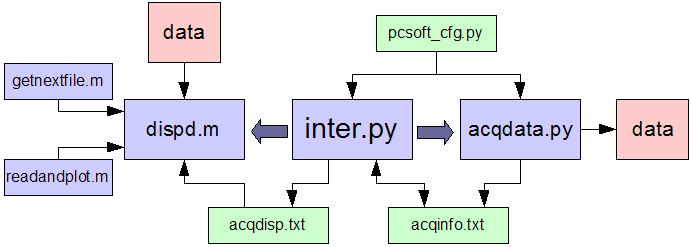
\includegraphics[scale=0.65]{../drawings/pcsoft_files_diagram.png}
\end{center}
\caption[PC Software Files Block Diagram]{Block diagram of the PC Software files. Blocks in blue
indicate files in which execution of code occurs. Blocks in green are data/control files. Blocks
in red represent acquired data.}
\label{fig:pcsoft files diagram}
\end{figure}


\subsubsection[inter.py]{inter.py}
This is the main hub of the PC Software subsystem. In addition to generating and displaying the 
main graphical front-end seen by the user, it performs the following tasks:

\begin{itemize}
\item Initiates the data acquisition process by launching the data acquisition software in a 
sub-process and communicating with it via sockets.
\item Enables user to specify configuration bits for the data acquisition hardware, including 
whether the input signal is analog or digital; allows user to enable/disable output.
\item Allows user to associate a mnemonic label with a data acquisition.
\item Provides to user a way to delete, scroll through and search previously saved data.
\item Enables on-demand data plotting by providing a method of displaying an acquisition; launches 
the GNU Octave data display script in a separate subprocess when such input has occurred.
\end{itemize}


A screenshot of the interface that inter.py creates is shown in Figure \ref{fig:pcsoft inter ss}. The
UI consists of three different areas: the Data Acquisition frame, the Data Display frame and the
Control Interface frame.

\begin{figure}[bhp]
\begin{center}
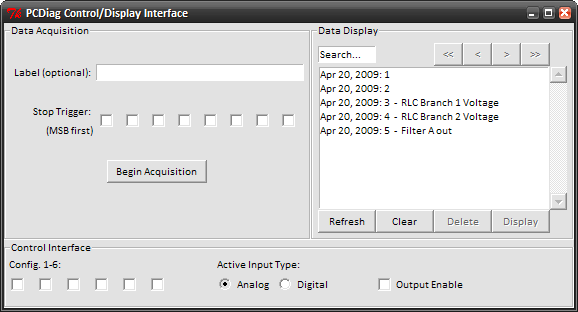
\includegraphics[scale=0.6]{../drawings/pcsoft_inter_ss.png}
\end{center}
\caption[PC Software Interface Screenshot]{Screenshot of the PC Software GUI front-end.}
\label{fig:pcsoft inter ss}
\end{figure}


The data acquisition process is initiated in the Data Acquisition frame by clicking on the 
``Begin Acquisition'' button. A series of checkboxes labeled ``Stop Trigger'' allows the user
 to define the bit pattern that the data acquisition software will detect to terminate the 
acquisition session. An optional label entry field allows the user to associate a label with 
an acquisition session as a means of organizing data that is captured by the software.


The Control Interface frame provides the user with configuration options for the acquisition
hardware. A group of 6 checkboxes labeled ``Config 1-6'' are general configuration options for
the currently active input. Two radio buttons provide control over the type of input signal,
and a last checkbox allows the user to enable or disable output.


The Data Display frame provides the user with an interface for managing previously acquired
data. The acquisition list displays and orders acquisitions by date and number. Labels are
displayed for acquisitions that have them. Because a user may eventually accumulate hundreds
of acquisitions, acquisitions are broken up into ``pages,'' which ensures that not too many
are displayed at one time. Four arrow buttons on the top right allow the user to go to the first 
page, the previous page, the next page or the last page. Four buttons at the bottom of the 
acquisition allow the user to perform various actions:

\begin{itemize}
\item ``Refresh'' - Refreshes the list.
\item ``Clear'' - Deletes every acquisition in the acquisition list.
\item ``Delete'' - Deletes only the selected acquisitions out of the list.
\item ``Display'' - Provides on-demand data plotting by launching the GNU Octave data display script.
\end{itemize}


\subsubsection[acqdata.py]{acqdata.py}
Acqdata.py is the data acquisition software. It is launched in a separate process when a user 
clicks on the ``Begin Acquisition'' button in the interface. This program quite simply reads
opens a connection with the serial port and reads data in continuously into a buffer until the 
stop trigger is detected. To avoid a possible buffer overflow, data is written to a binary file
when the buffer fills. In the case of large acquisitions, acqdata.py will break the acquisition 
output up into several parts. Output file names follow a format: \\\ \\
DDMonYY\_Np \\\ \\

where ``DD'' is the two-digit date of the acquisition, ``Mon'' is a three letter abbreviation 
of the month of the acquisition, ``YYYY'' is the four-digit year of the acquisition, ``N'' is 
the number of the acquisition on the date it occurred and ``p'' is the letter of the acquisition part, starting with `a' and continuing through `z'. 

\subsubsection[pcsoft\_cfg.py]{pcsoft\_cfg.py}

\subsubsection[acqinfo.txt]{acqinfo.txt}

\subsubsection[acqdisp.txt]{acqdisp.txt}

\subsubsection[dispd.m]{dispd.m}

\subsubsection[getnextfile.m]{getnextfile.m}

\subsubsection[readandplot.m]{readandplot.m}



\fancyfoot[R]{}
\begin{appendix}
% The beginning of the appendix.
% Documents that are part of the appendix need to go here.
% All datasheets for our project.
\chapter{Datasheets}
% Analog MUX used in signal conditioner

\includepdf[pages=2-8]{../ref/CD4067.pdf}

%WT32

\includepdf[pages=-]{../ref/WT32_Datasheet.pdf}
% 74LS gates, 244 is unused.
%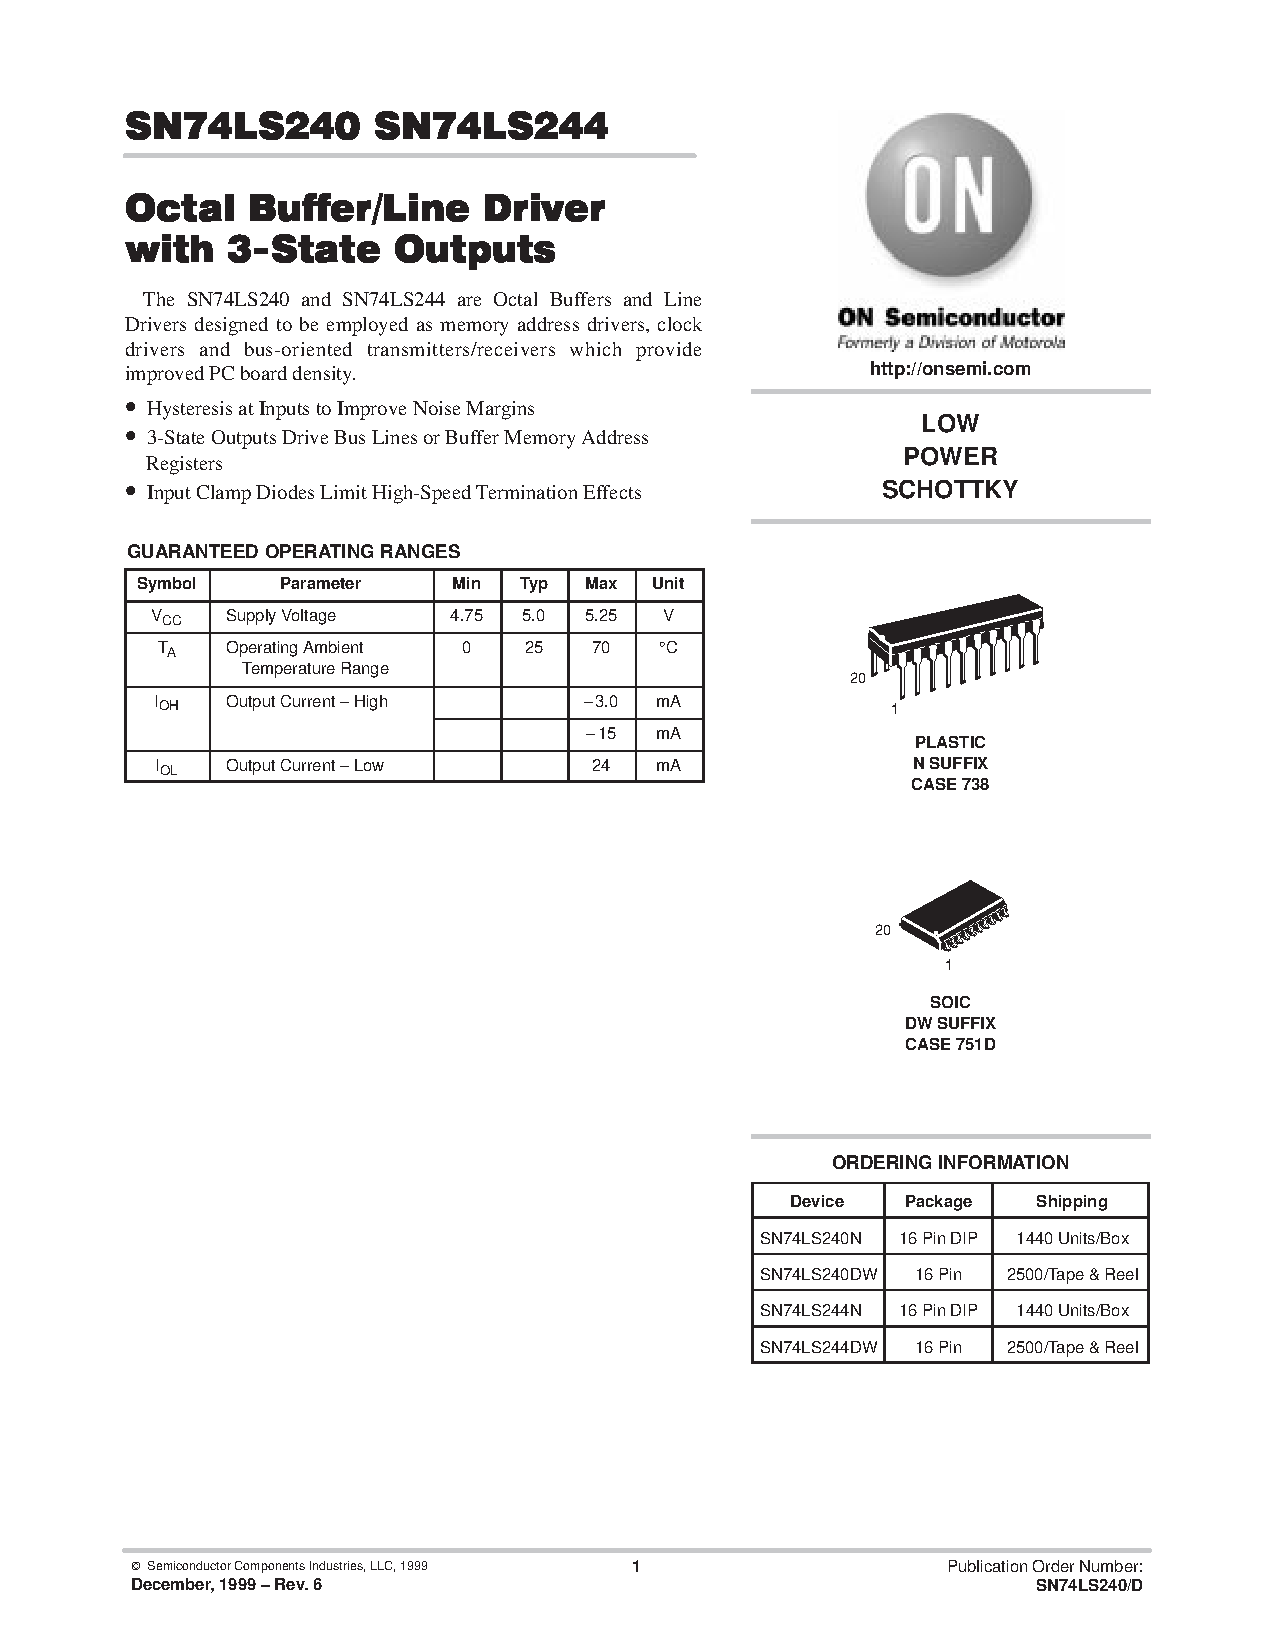
\includepdf[pages=-]{../ref/74LS244.pdf}
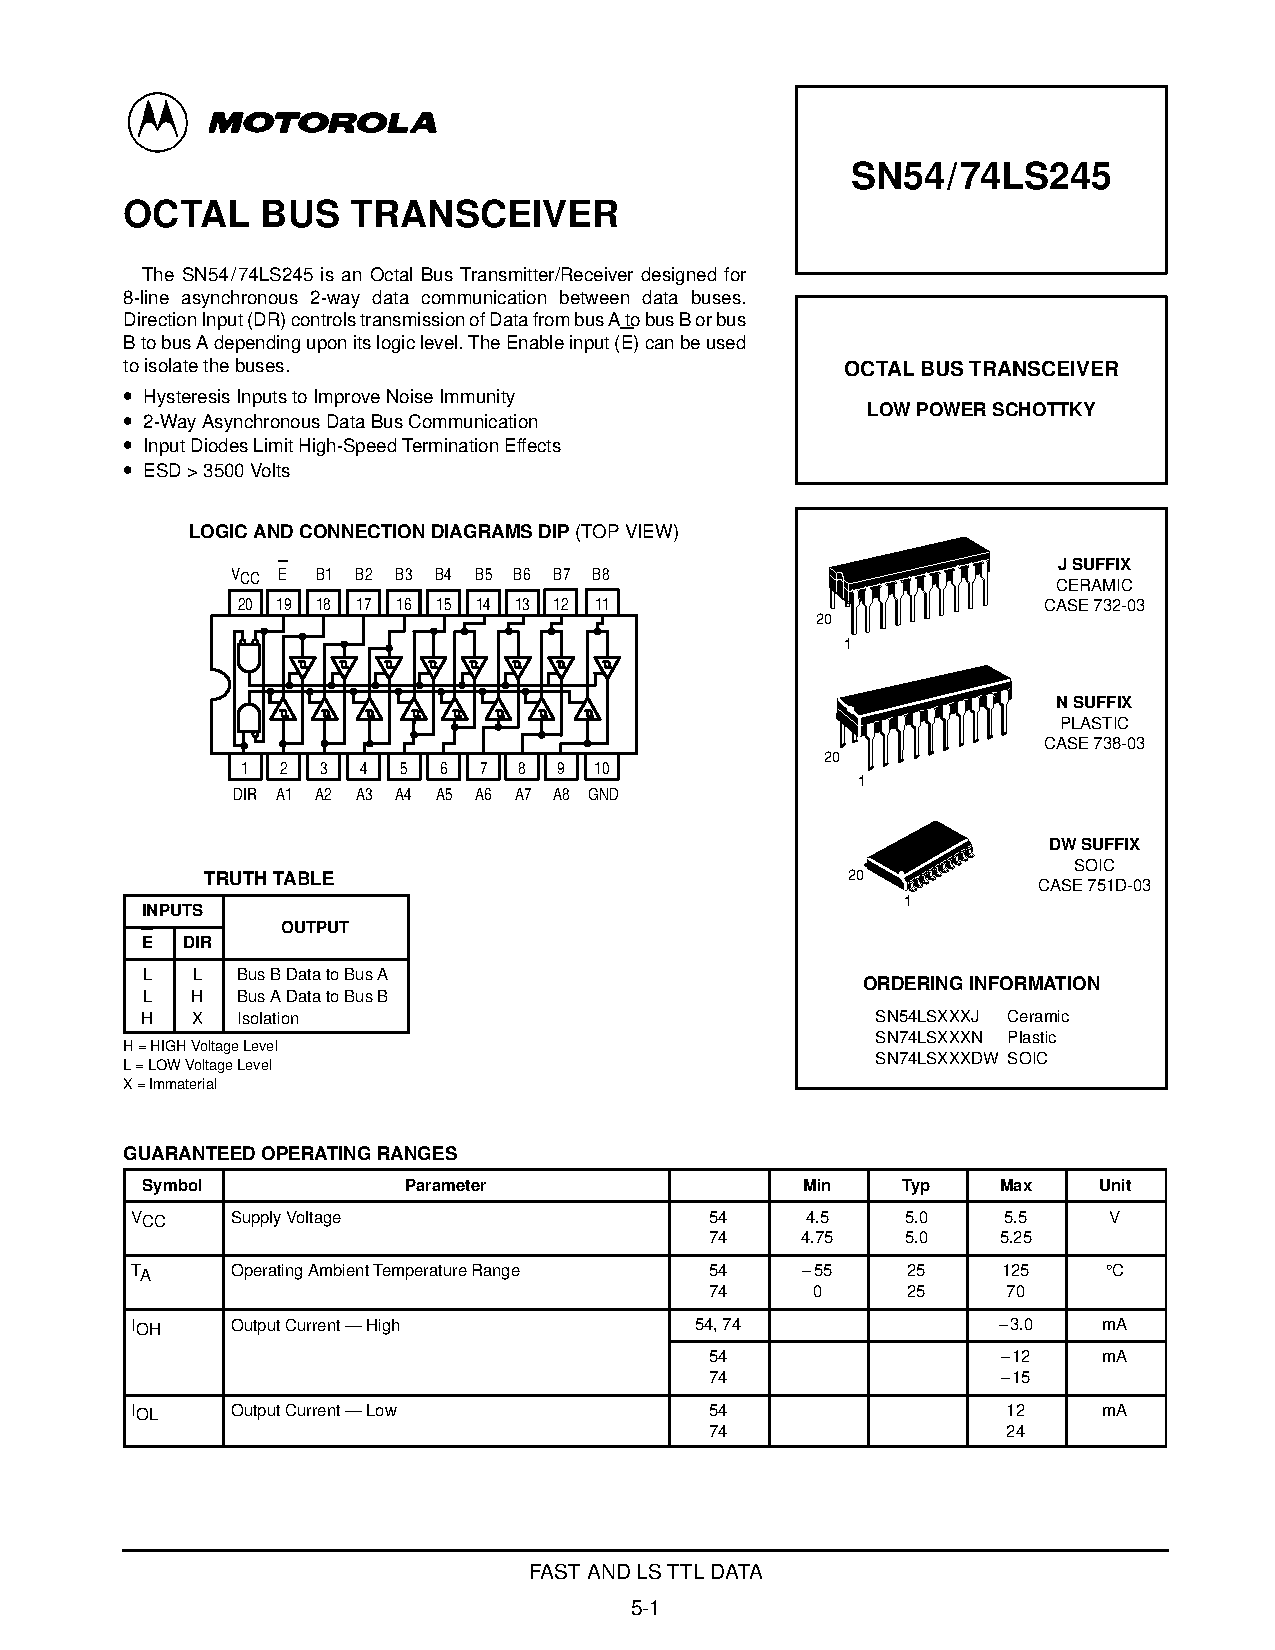
\includepdf[pages=-]{../ref/74LS245.pdf}
% 74*1160 datasheet, part is unused.
%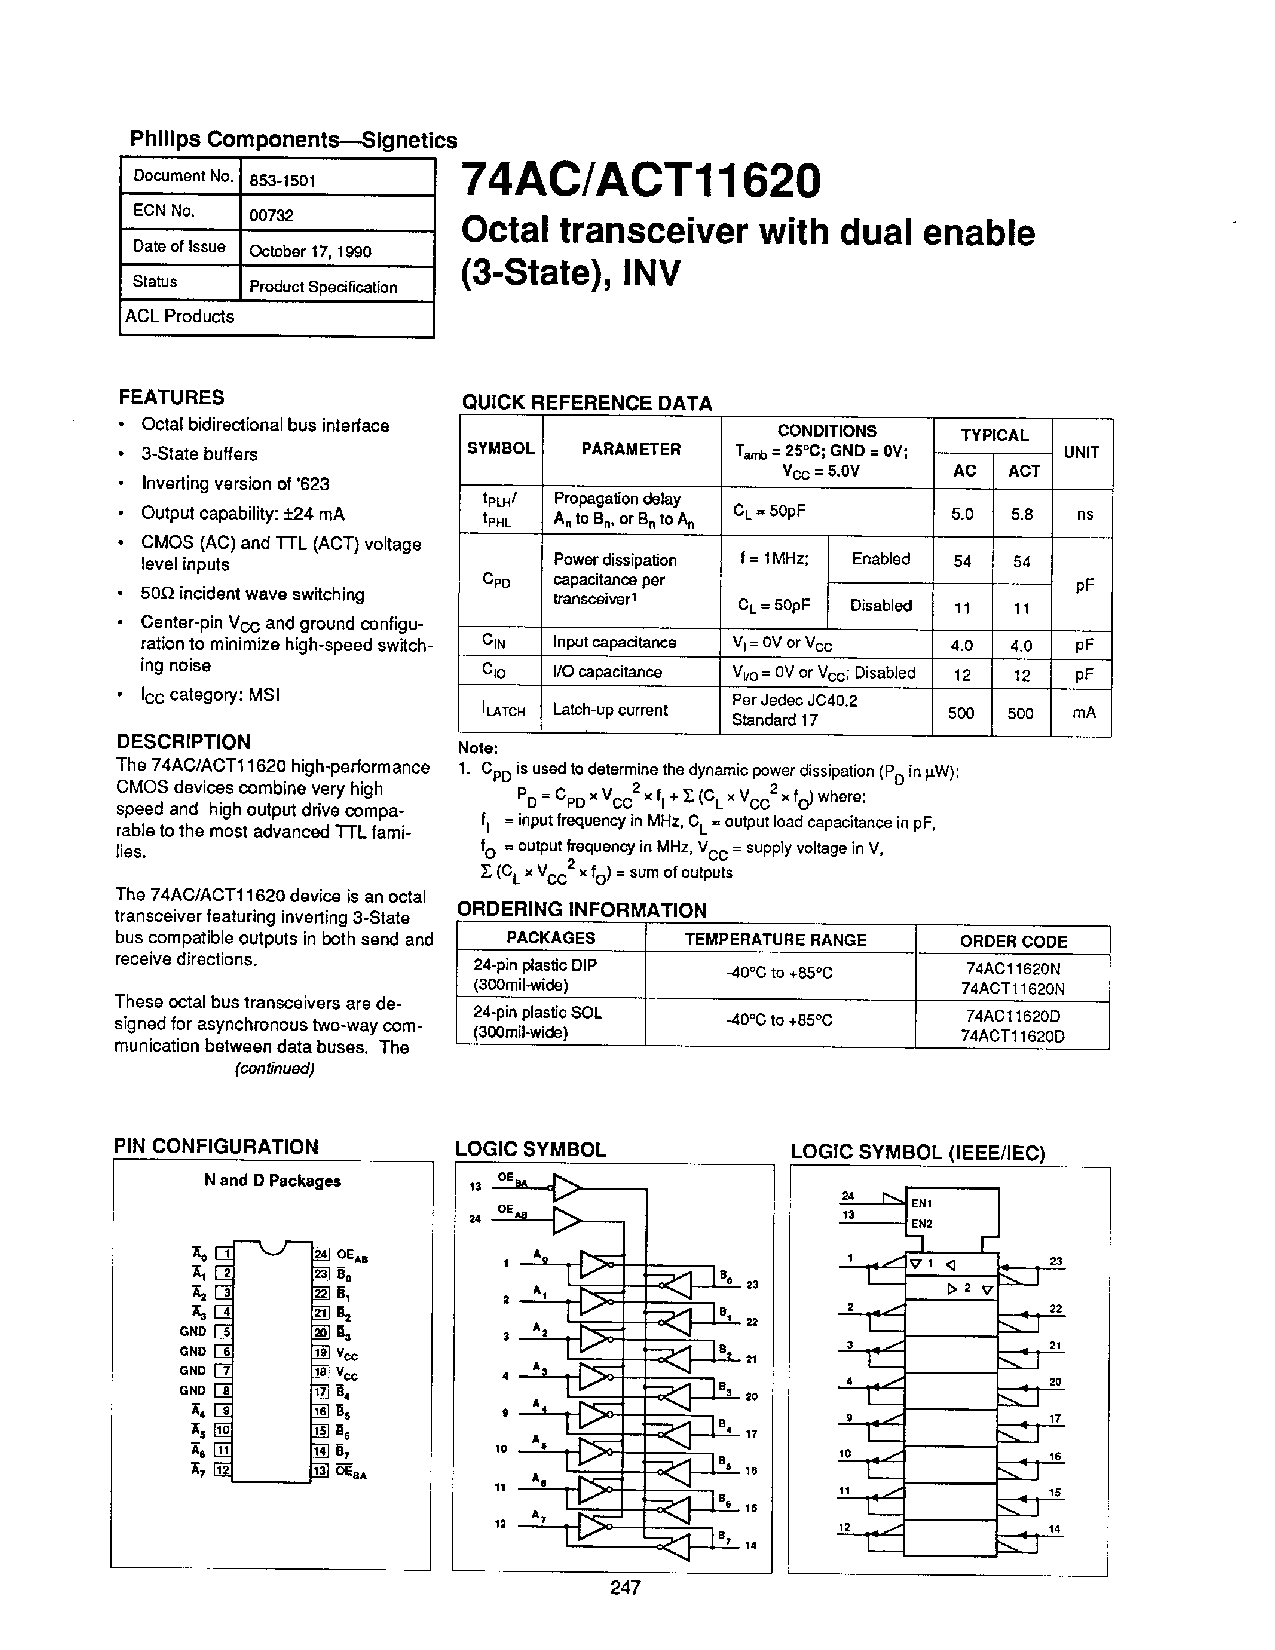
\includepdf[pages=-]{../ref/74AC11620.pdf}

%ADC
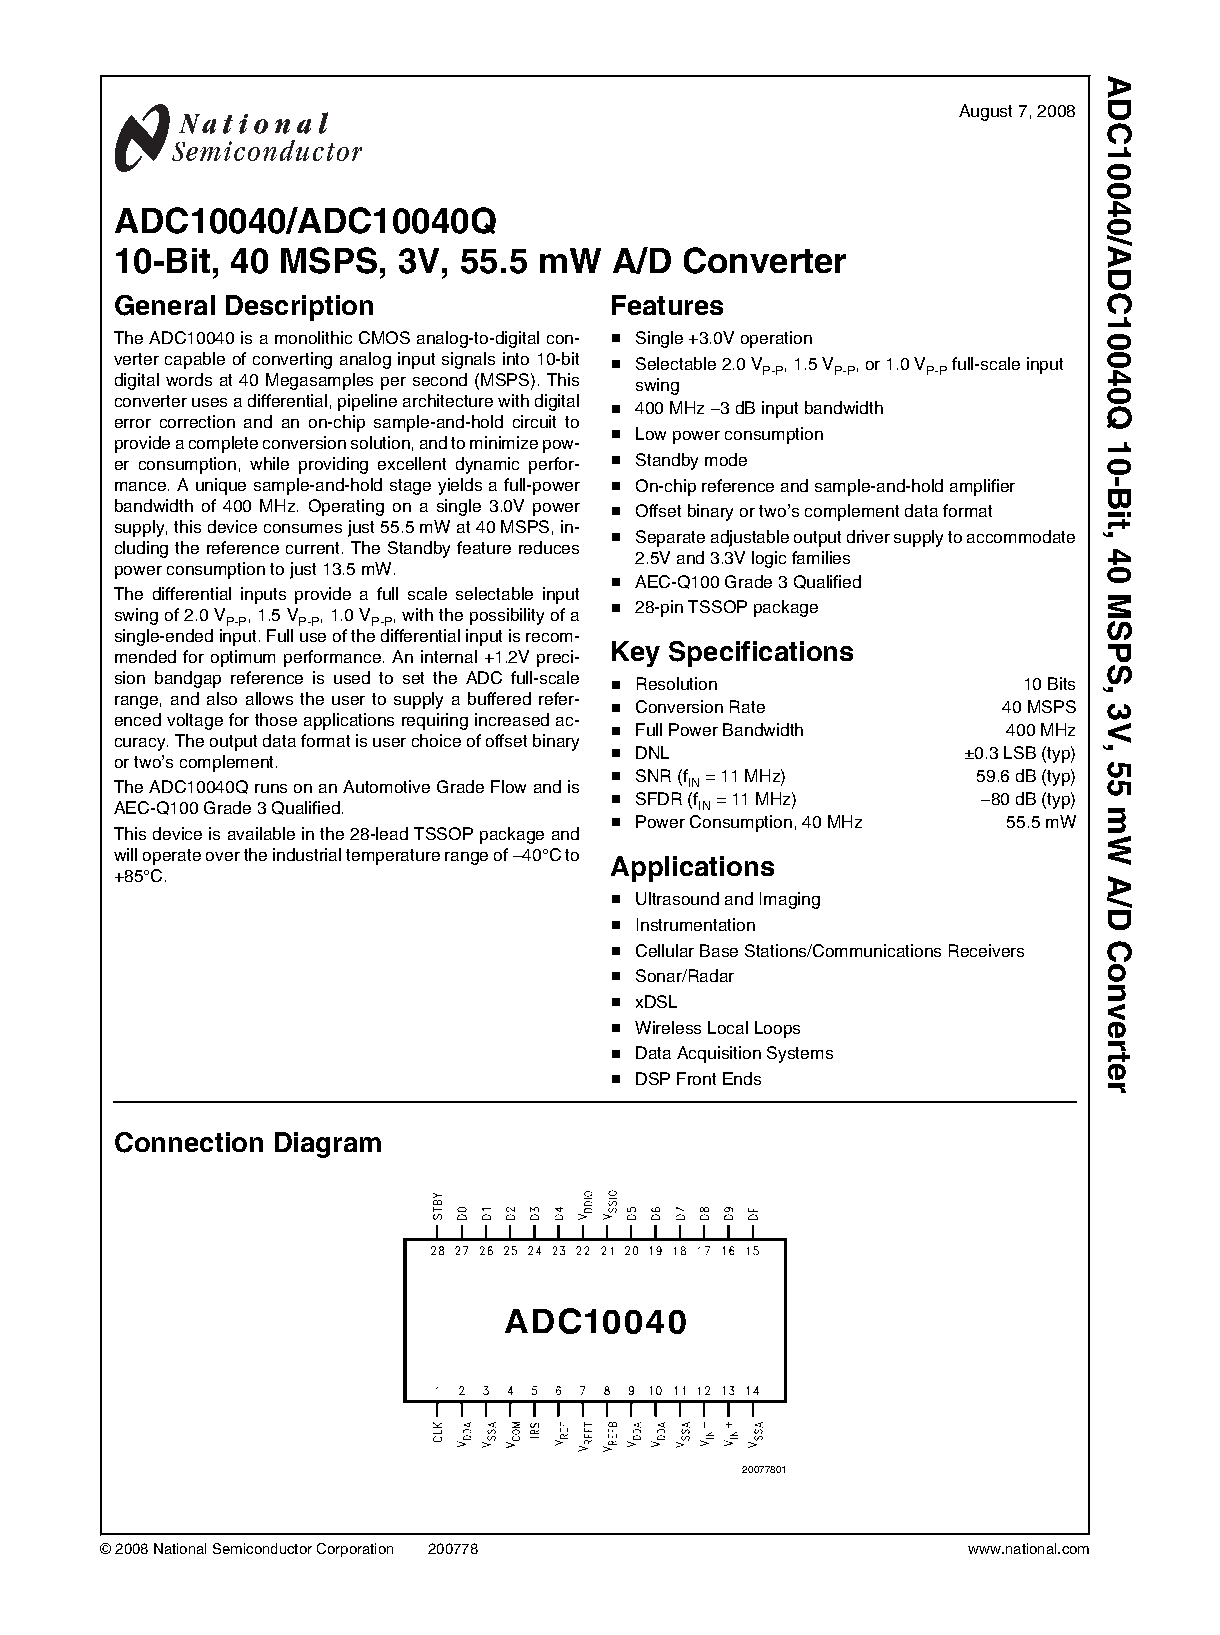
\includepdf[pages=-]{../ref/ADC10040.pdf}

%MAX step-ups
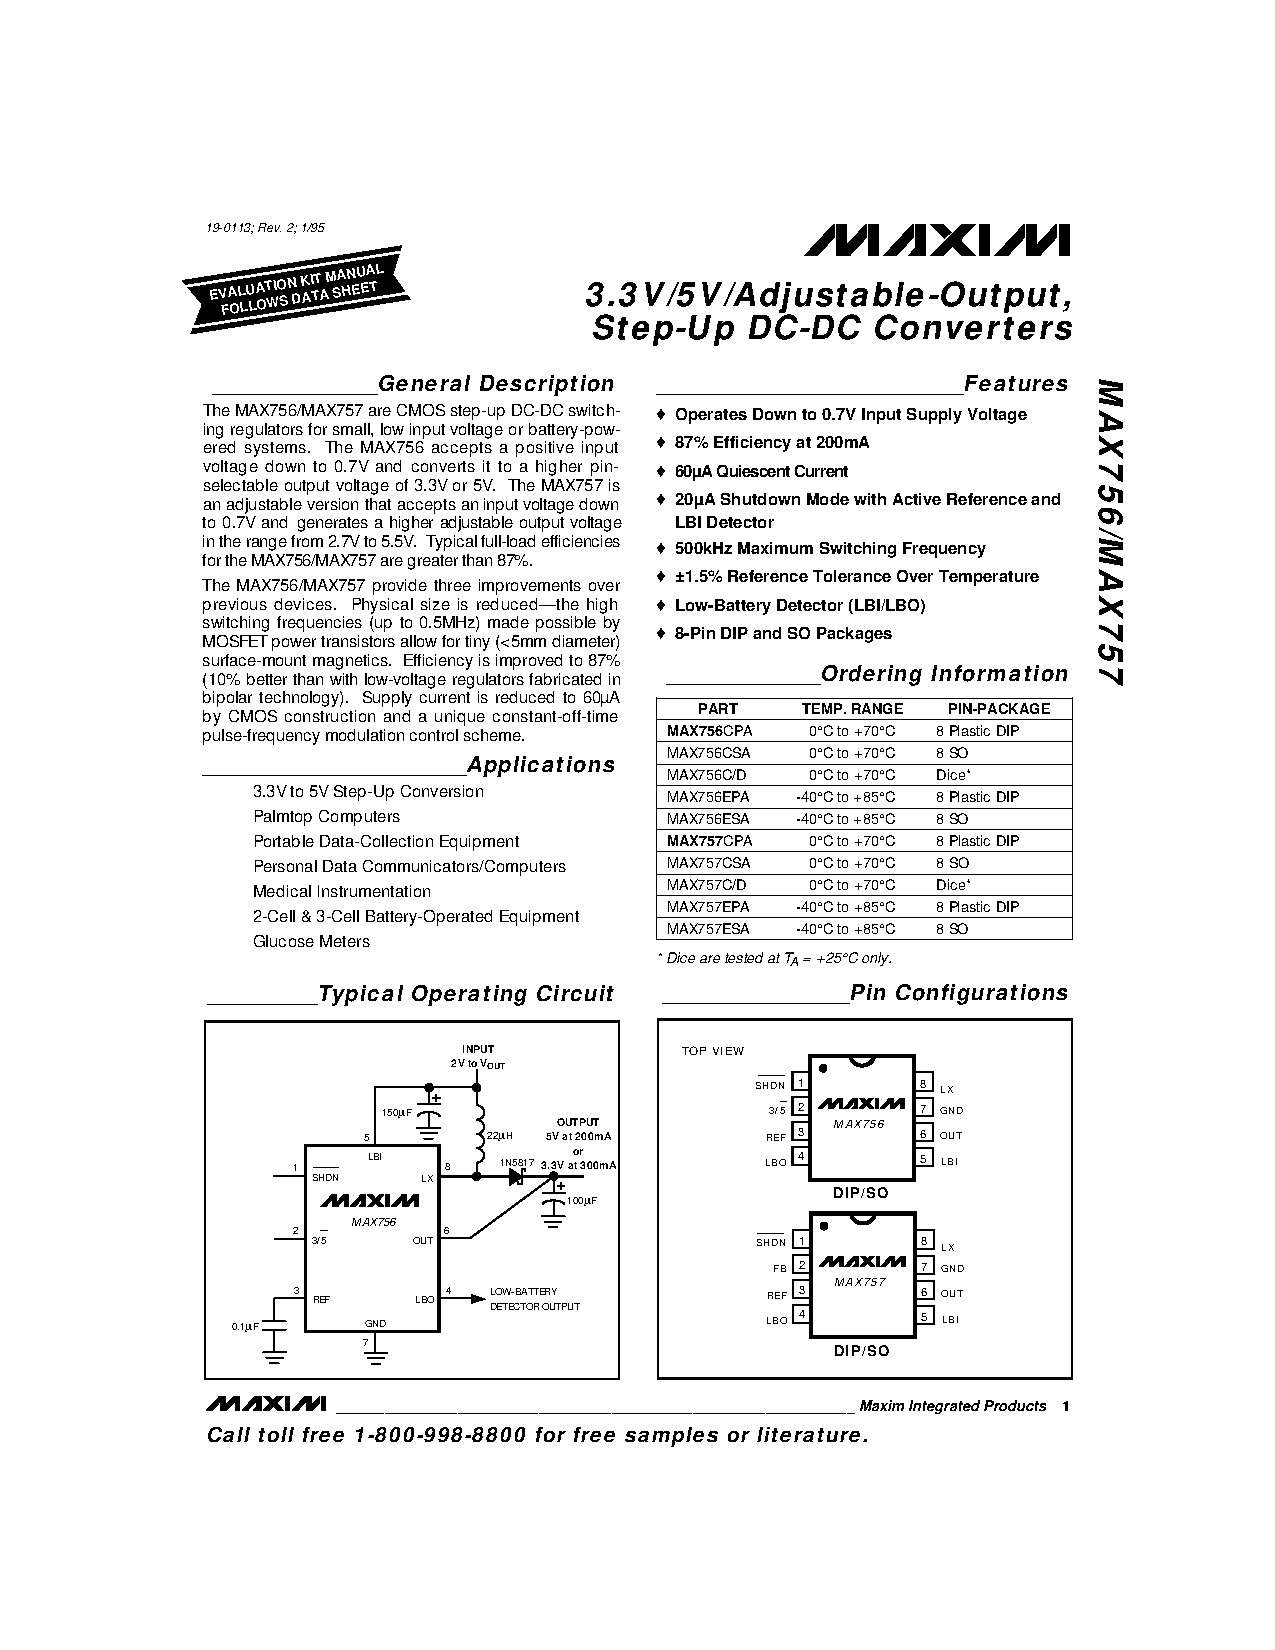
\includepdf[pages=-]{../ref/MAX756-MAX757.pdf}



% All code listings for our project.
\chapter{Software Listings}
%Put all printouts of code listings here.
\lstset{numbers=left, tabsize=2, breakatwhitespace=true}
\lstset{columns=fullflexible}
\lstset{breaklines=true}
\section[Controller Source]{Microcontroller Source Code}

\subsection{Main Control Unit}\index{MCU}\index{Main Control Unit}
\lstset{language=c}
\lstinputlisting[caption=Main Control Unit Header, label=lst:mcu_h]{../src/mcu/main_control.h}
\lstinputlisting[caption=Main Control Unit, label=lst:mcu_c]{../src/mcu/main_control.c}

\subsection{Serial Control Unit}\index{SCU}\index{Serial Control Unit}
\lstinputlisting[caption=Serial Control Unit, label=lst:scu_c]{../src/mcu/usart.c}

\subsection{Common Utilities}
\lstinputlisting[caption=SPI Interface Functions, label=lst:spi_c]{../src/mcu/spi_util.c}
\lstinputlisting[caption=USART Interface Functions, label=lst:usart_c]{../src/mcu/usart_util.c}
\lstinputlisting[caption=Common Defines, label=lst:common_h]{../src/mcu/control_defines.h}

\section{Host PC Software}
\lstset{language=python}
\subsection{Display/Control Interface}
\lstinputlisting[caption=Display/Control Interface, label=lst:inter]{../src/pcsoft/inter.py}

\subsection {Data Acquisition}
\lstinputlisting[caption=Data Acquisition,label=lst:acqdata]{../src/pcsoft/acqdata.py}

\subsection {PC Software Configuration}
\lstinputlisting[caption=Software Configuration, label=lst:pcsoft\_cfg]{../src/pcsoft/pcsoft_cfg.py}

\subsection{Data Display}
\lstset{language=matlab}
\lstinputlisting[caption=Matlab/Octave Data Display,label=lst:dispd]{../src/pcsoft/dispd.m}
\lstinputlisting[caption=Matlab/Octave Get Next File, label=lst:getnextfile]{../src/pcsoft/getnextfile.m}
\lstinputlisting[caption=Matlab/Octave Read/Plot Data, label=lst:readandplot]{../src/pcsoft/readandplot.m}

\fancyfoot[R]{}

% Recommended vendor list.
%add vendors here for specific parts
\section{Recommended Vendors}

\begin{itemize}
\item For the ATMega8515L
\begin{enumerate}
	\item Farnell (\url{http://www.farnell.com/uk})
	\item Futurelec (\url{http://www.futurelec.com})
	\item Jameco Electronics, PDIP only (\url{http://www.jameco.com})
\end{enumerate}

\item For general ICs (74-series):
\begin{enumerate}
	\item Jameco Electronics (\url{http://www.jameco.com})
	\item Futurelec (\url{http://www.futurelec.com})
	\item Jameco Electronics, PDIP only (\url{http://www.jameco.com})
\end{enumerate}
\end{itemize}

\fancyfoot[R]{}
\section{Engineering Drawings}
\subsection{Data Acquisition Unit Datapath}
\label{sch:datapath}
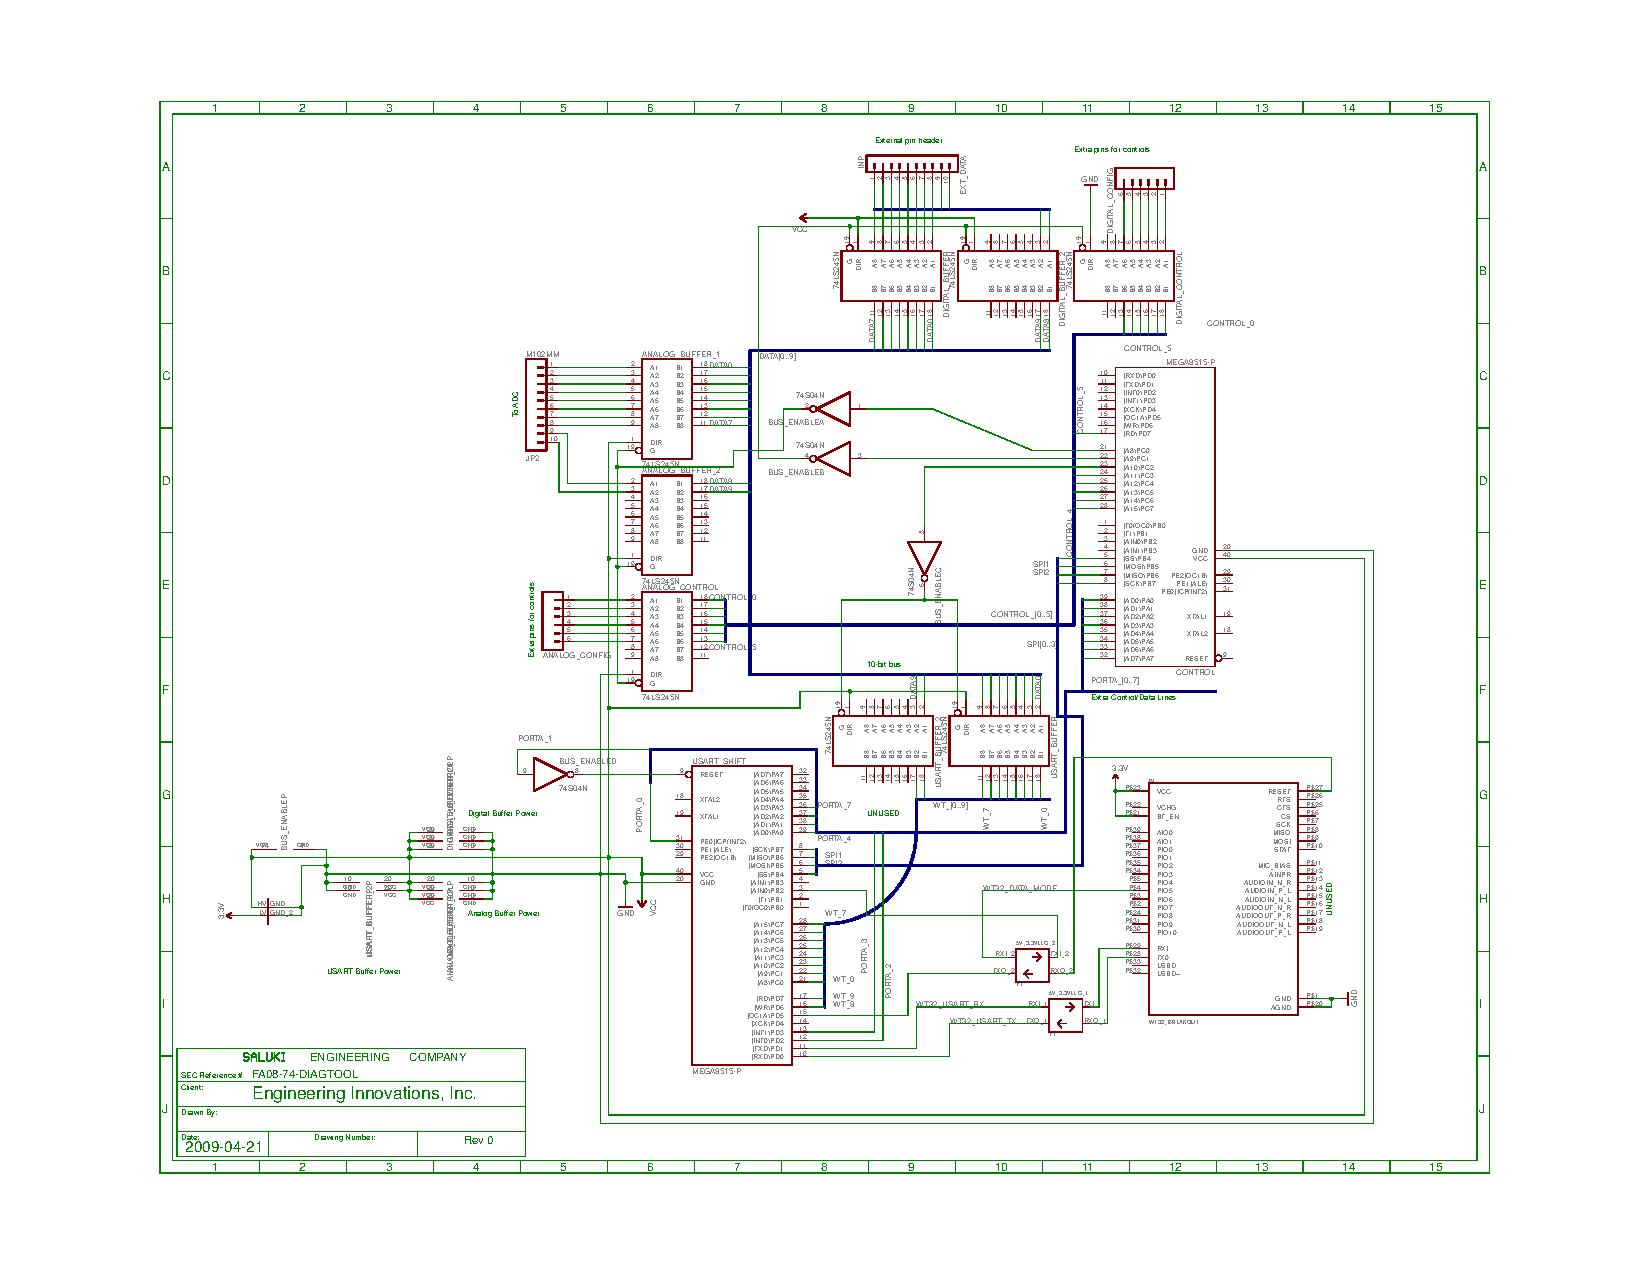
\includepdf{acquunit.pdf}

\subsection{Analog Input Amplification Circuit}
\label{sch:signal amp}
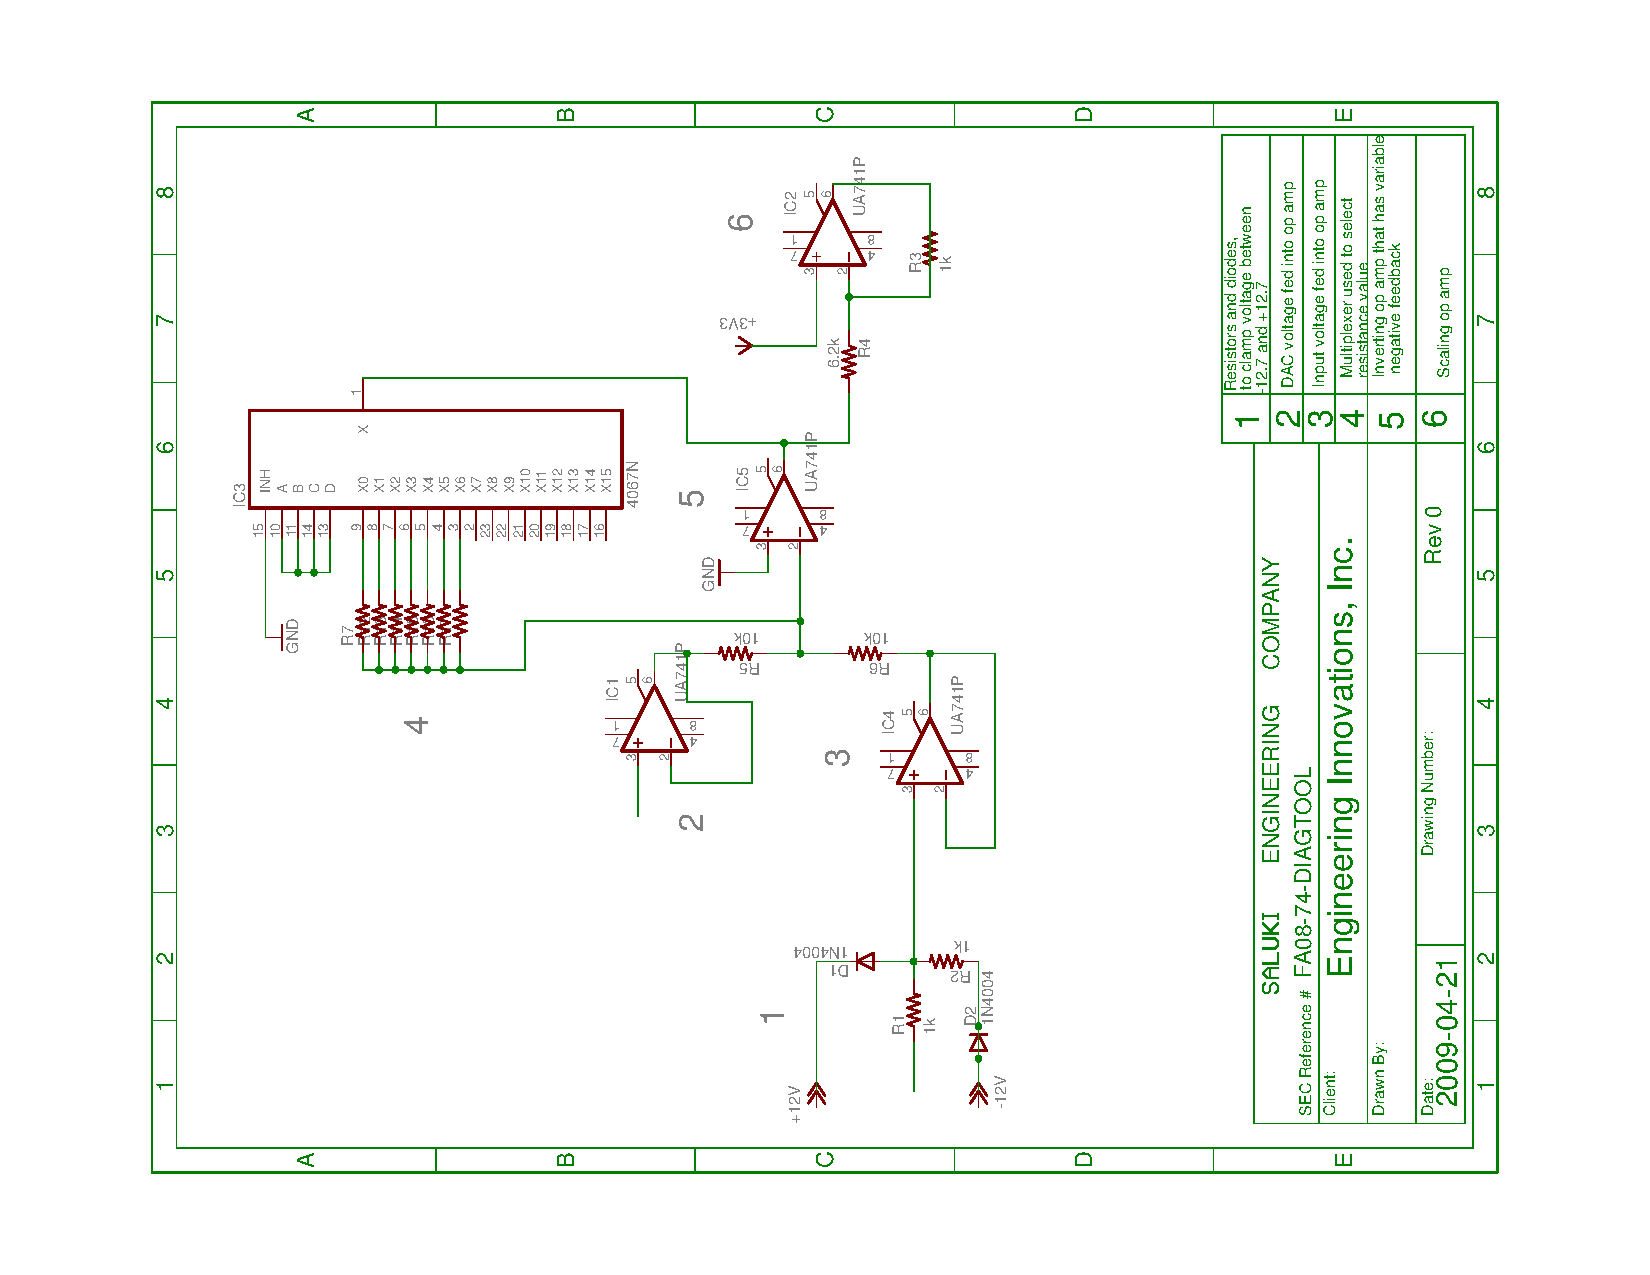
\includepdf{amplification.pdf}


\addcontentsline{toc}{chapter}{List of Figures}
\listoffigures
\addcontentsline{toc}{chapter}{List of Tables}
\listoftables
\end{appendix}

\addcontentsline{toc}{chapter}{Bibliography}
\bibliographystyle{ieeetr}
\bibliography{citations}
\printindex
\end{document}
